\chapter{OpenSBLI - extension to thermochemical nonequlibrium}\label{chapter:numerical_methods}

The research employs the in-house open-source platform \textit{OpenSBLI}, a finite-difference solver for compressible fluid dynamics designed to target a wide range of computational hardware \citep{LusherEtAl2025, LusherJammySandham2021}. OpenSBLI is an automatic code-generation framework with a high-level Python front end and a low-level C backend, coupled to the \gls{OPS} embedded domain-specific library \citep{RegulyMudaligeGiles2018}. The code-generation approach enables a separation of concerns: the physical problem and numerical schemes are decoupled from their parallel implementation, allowing users to focus on their area of expertise whilst maintaining a reduced and more maintainable code base. The governing equations are expressed in Einstein index notation within the Python front end, where the software uses the symbolic computation library \texttt{SymPy} to perform algebraic manipulations and discretise the equations into low-level C code. This symbolic manipulation enables performance optimisations that would not be feasible in hand-written codes \citep{JammyEtAl2016}.

\begin{figure}[t]
    \centering
    \includegraphics[width=12.0cm]{resources/figures/opensbli/schematic_2025_opebsbli_structure.pdf}
    \caption{An overview of the structure of the OpenSBLI system showcasing the linkage between the core classes \citep{LusherJammySandham2021}, where the HPC architecture conversion is handled by the OPS translator.}
    \label{figure:opensbli_structure}
\end{figure}

OpenSBLI converts high-level mathematical descriptions into low-level C code that calls \gls{OPS} library functions~\citep{RegulyMudaligeGiles2018}, as shown in Figure~\ref{figure:opensbli_structure}. The \gls{OPS} library is a programming abstraction for multi-block structured mesh applications designed to achieve near-optimal performance on modern hardware. The C code produced by OpenSBLI can be translated automatically into multiple parallel programming paradigms including MPI, OpenMP, CUDA, OpenCL, and OpenACC, enabling efficient execution of large-scale \gls{DNS} on HPC clusters. Previous work has demonstrated that this system is able to match or exceed the performance of hand-written code \citep{MudaligeEtAl2019}. Within the Python setup file, the user specifies the numerical scheme, governing equations, initial and boundary conditions, and grid coordinates. Equations are implemented through the \texttt{SymPy} equation class, enabling concise formulations with automatic symbolic substitutions that reduce errors and improve readability. The full set of governing equations is also written to a LaTeX file for straightforward debugging. Grid coordinates and initial conditions may be defined analytically or imported from external files, whilst boundary conditions are prescribed on each domain surface. Upon execution of the setup file, the problem is discretised and core simulation classes are generated as computational kernels in the \gls{OPS}-C language, which are then translated into architecture-specific implementations. This structure ensures that problems defined in a single high-level setup file can be executed across diverse parallel architectures without manual code modification.

In the present work, the existing OpenSBLI framework has been extended to incorporate thermochemical nonequilibrium physics with various transport and chemical models. This required transitioning from the conventional non-dimensional formulation to a fully dimensional framework and substantial modifications to the source code to accommodate additional governing equations and energy modes. The framework now supports multiple high-order numerical schemes for both spatial discretisation and temporal integration, with their implementations and performance characteristics detailed in this section.

% To enable efficient, high-fidelity simulations on modern hardware, \texttt{OpenSBLI} provides an in-house open-source framework for the automatic generation of finite-difference solvers for compressible flows \citep{Jacobs2017, lusher2021}. The platform combines a high-level Python front end with a low-level C backend and is coupled with the Oxford Parallel Structured (OPS) embedded domain-specific language (DSL) library \citep{Reguly_et_al_2018}, which enables the generated source code to target multiple parallel architectures. The governing equations are specified in index notation within the Python front end, where the software uses Python’s symbolic computation library, SymPy, to manipulate expressions and discretise the equations into optimised C code. Some of the major advantages of such a method include: separation of concerns, where the physical problem in question is “separated” from the numerical schemes and their parallel implementations, reduced size of the code base as compared to static codes, improving tractability and maintainability and enhancing performance as opposed to static written codes\citep{jammy2016}. The main purpose of OpenSBLI is the conversion from high-level code to low level C code which entails writing the equations utilising the OPS library functions. The OPS library is a framework for multi-block structured mesh targeting parallel architectures which can apply a wide range of optimisations to multi-block structured meshes and deliver near optimal performance on modern hardware. The APIs of the OPS-DSL framework enable the definition of blocks, datasets, halos, and a plethora of computational definitions, providing intuitive coding framework that is similar to a traditional single-threaded sequential code. Therefore, the C code produced by OpenSBLI is further translated to a variety of parallel programming paradigms, including MPI, OpenMP, CUDA, OpenCL and OpenACC, expeditiously providing an implementation of large-scale Direct Numerical Simulations (DNS) on HPC clusters . The general structure of OpenSBLI is shown in the figure below, where the integrations between key classes of software and the OPS-DSL library are clearly highlighted; here, the python code is written at the top, where the OpenSBLI performs necessary manipulations to couple the output with the OPS library. A detailed literature of 

% \begin{enumerate}
%     \item Talk about OpenSBLI, how it works 
%     \item Structure figure
%     \item changes and challenges to incporate real gas effects: feature for efficient loops in the simulations, new boundary conditions, Jacobian, RoeAveraging, changes to accomodate dimensional simulations. 
% \end{enumerate}

% \section{Spatial and temporal derivatives}

% Spatial derivatives in OpenSBLI are generated through central finite-difference schemes of arbitrary even order \citep{LusherEtAl2025,RegulyMudaligeGiles2018}. In the present work, a fourth-order central scheme is employed for convective, viscous, and metric derivatives, given for a uniform spacing $\Delta x$ by
% \begin{equation}
%     \pdv{f}{x} \approx \frac{-f_{i+2} + 8 f_{i+1} - 8 f_{i-1} + f_{i-2}}{12 \,\Delta x}.
% \end{equation}
% For wall-bounded domains, one-sided formulations following~\cite{CarpenterNordstromGottlieb1999} are used near the boundaries, with the first four points modified by optimised coefficients to preserve fourth-order accuracy. Consistency between the interior central stencil and the one-sided boundary closures prevents spurious errors associated with order mismatches. An alternative fourth-order scheme due to \cite{Ekaterinaris2005} is also available in OpenSBLI and has been shown to be computationally more efficient, though the present study adopts the Carpenter-type closure for robustness.

\section{Spatial and Temporal Derivatives}
\subsection{Central Differencing}
Spatial derivatives in OpenSBLI are generated through central finite-difference schemes of arbitrary even order, with implementations available for fourth-, sixth-, eighth-order and higher formulations \citep{LusherEtAl2025,RegulyMudaligeGiles2018}. The framework applies these schemes identically in both non-dimensional and dimensional formulations, maintaining consistency across different problem types. In the present work, a fourth-order central scheme is employed for all spatial derivatives, including convective flux terms, viscous flux terms, and metric derivatives arising from coordinate transformations. For a uniform computational spacing $\Delta x_j$ in the $j$-direction, the spatial derivative is approximated as
\begin{equation}
    \pdv{f}{x_j} \approx \frac{f_{i-2} - 8 f_{i-1} + 8 f_{i+1} - f_{i+2}}{12 \,\Delta x_j}
\end{equation}
at interior points of the computational domain. To improve numerical stability and prevent odd-even decoupling, Laplacian terms appearing in the viscous fluxes are expanded explicitly, and one-sided derivative formulations are employed at all domain boundaries, excluding periodic boundaries where the central stencil can be applied directly.

Wall-bounded simulations require special treatment near solid surfaces where the standard central stencil cannot be applied due to insufficient grid points. OpenSBLI incorporates one-sided derivative schemes based on the formulations of \cite{CarpenterNordstromGottlieb1999} and \cite{Ekaterinaris2005}. Both approaches maintain fourth-order accuracy at the boundaries, which is essential to prevent spurious numerical errors arising from order mismatches when coupling schemes of different formal accuracy within the same domain. The Carpenter formulation constructs a first-derivative operator $\mathbf{D}$ through the relation
\begin{equation}
    \mathbf{D}\mathbf{f} = \frac{1}{\Delta x_j} \mathbf{P}^{-1} \mathbf{Q} \mathbf{f},
\end{equation}
where $\mathbf{f}$ represents a vector containing the boundary point and five interior flow variable values in the wall-normal direction. The matrices $\mathbf{P}$ and $\mathbf{Q}$ contain carefully optimised coefficients that preserve fourth-order accuracy whilst satisfying the summation-by-parts property, which ensures discrete conservation of energy and enhances numerical stability in wall-bounded configurations. The Ekaterinaris scheme provides an alternative approach with approximately 10\% reduced computational cost due to more compact stencils that require fewer grid points. The present work employs the Carpenter scheme for its robust stability properties. At the $i=0$ and $i=N-1$ boundaries, the first derivatives with respect to $x_j$ are computed as \begin{align}
    f'_0 &= \frac{1}{12\Delta x_j} \left(-25 f_0 + 48 f_1 - 36 f_2 + 16 f_3 - 3 f_4\right), \\[0.8em]
    f'_1 &= \frac{1}{12\Delta x_j} \left(-3 f_0 - 10 f_1 + 18 f_2 - 6 f_3 + f_4\right), \\[0.8em]
    f'_{N-2} &= \frac{1}{12\Delta x_j} \left(-f_{N-5} + 6 f_{N-4} - 18 f_{N-3} + 10 f_{N-2} + 3 f_{N-1}\right), \\[0.8em]
    f'_{N-1} &= \frac{1}{12\Delta x_j} \left(3 f_{N-5} - 16 f_{N-4} + 36 f_{N-3} - 48 f_{N-2} + 25 f_{N-1}\right),
\end{align}
where the prime notation denotes differentiation with respect to $x_j$. Second derivatives at the two points nearest to boundaries are evaluated as
\begin{align}
    f''_0 &= \frac{35 f_0 - 104 f_1 + 114 f_2 - 56 f_3 + 11 f_4}{12\Delta x_j^2}, \\[0.8em]
    f''_1 &= \frac{11 f_0 - 20 f_1 + 6 f_2 + 4 f_3 - f_4}{12\Delta x_j^2}.
\end{align}

For flows over complex geometries, OpenSBLI supports generalised coordinate transformations following the methodology of \cite{ZhangZhang2022}. The transformation maps the physical coordinates $(x_0, x_1, x_2)$ to a computational system $(\xi, \eta, \zeta)$ such that
\begin{equation}
    \xi = \xi(x_j), \quad \eta = \eta(x_j), \quad \zeta = \zeta(x_j), \quad j = 0, 1, 2,
\end{equation}
which allows derivatives in physical space to be expressed in terms of computational coordinates using the chain rule:
\begin{equation}
    \pdv{}{x_j} = \xi_{x_j} \pdv{}{\xi} + \eta_{x_j} \pdv{}{\eta} + \zeta_{x_j} \pdv{}{\zeta},
\end{equation}
where $\xi_{x_j} = \partial\xi/\partial x_j$, $\eta_{x_j} = \partial\eta/\partial x_j$, and $\zeta_{x_j} = \partial\zeta/\partial x_j$ are the metric coefficients that quantify how the grid transforms between physical and computational spaces. The Jacobian of the transformation is defined as
\begin{equation}
    J = \frac{\partial(\xi, \eta, \zeta)}{\partial(x_0, x_1, x_2)} = 
    \begin{vmatrix}
        \xi_{x_0} & \xi_{x_1} & \xi_{x_2} \\
        \eta_{x_0} & \eta_{x_1} & \eta_{x_2} \\
        \zeta_{x_0} & \zeta_{x_1} & \zeta_{x_2}
    \end{vmatrix},
\end{equation}
with its inverse
\begin{equation}
    \frac{1}{J} = \frac{\partial(x_0, x_1, x_2)}{\partial(\xi, \eta, \zeta)} = 
    \begin{vmatrix}
        x_{0,\xi} & x_{0,\eta} & x_{0,\zeta} \\
        x_{1,\xi} & x_{1,\eta} & x_{1,\zeta} \\
        x_{2,\xi} & x_{2,\eta} & x_{2,\zeta}
    \end{vmatrix},
\end{equation}
where $x_{i,\xi} = \partial x_i/\partial\xi$, and similarly for $\eta$ and $\zeta$. The metric terms are evaluated using the same fourth-order central scheme and boundary closures described above, ensuring consistency in the discretisation. In OpenSBLI, the coordinate transformation is applied symbolically to each derivative term through the SymPy framework. The derivatives are calculated on the uniform computational grid, and the metric coefficients are then incorporated into the derivative arrays during the time integration. This approach maintains conservation properties whilst enabling high-order accurate simulations on curvilinear meshes. In the present thermochemical nonequilibrium formulation, these discretisations are applied to the conservative state vector
\begin{equation}
    \mathbf{U} = \{\rho_{\text{N}_2}, \rho_{\text{O}_2}, \rho_{\text{NO}}, \rho_{\text{N}}, \rho_{\text{O}}, \rho u_0, \rho u_1, \rho u_2, \rho E, \rho e_v\},
\end{equation}
where $\rho_s$ denote species densities, $\rho u_i$ the momentum components, $\rho E$ the total energy, and $\rho e_v$ the vibrational energy. This unified treatment ensures that convective, viscous, and metric contributions are consistently discretised to fourth-order accuracy across all conserved variables, enabling stable and accurate large-scale \gls{DNS} of thermochemically reacting flows.

% The same central formulation is applied to viscous fluxes and to metric derivatives arising from curvilinear meshes, following the procedure of Rumsey and Biedron \citep{Rumsey2013}. The physical-space derivatives $(\partial/\partial x, \partial/\partial y, \partial/\partial z)$ are expressed in terms of the computational coordinates $(\xi,\eta,\zeta)$ using the chain rule,
% \begin{equation}
%     \pdv{}{x} = \xi_x \pdv{}{\xi} + \eta_x \pdv{}{\eta} + \zeta_x \pdv{}{\zeta}, \qquad
%     \pdv{}{y} = \xi_y \pdv{}{\xi} + \eta_y \pdv{}{\eta} + \zeta_y \pdv{}{\zeta}, \qquad
%     \pdv{}{z} = \xi_z \pdv{}{\xi} + \eta_z \pdv{}{\eta} + \zeta_z \pdv{}{\zeta},
% \end{equation}
% where the metric coefficients $(\xi_x,\xi_y,\xi_z,\dots)$ are computed consistently with the fourth-order discretisation. The Jacobian of the transformation ensures conservation properties are maintained, and contravariant velocities are used to assemble the fluxes in the transformed coordinate system.

% In the present thermochemical nonequilibrium formulation, these discretisations are applied to the conservative state vector
% \[
%     \{\rho_{\mathrm{N}_2}, \rho_{\mathrm{O}_2}, \rho_{\mathrm{NO}}, \rho_{\mathrm{N}}, \rho_{\mathrm{O}},
%     \rho u_0, \rho u_1, \rho u_2, \rho E, \rho e_v\},
% \]
% where $\rho_s$ denote species densities, $\rho u_i$ the momentum components, $\rho E$ the total energy, and $\rho e_v$ the vibrational energy. This unified treatment ensures that convective, viscous, and metric contributions are consistently discretised to fourth-order accuracy across all conserved variables, enabling stable and accurate large-scale DNS of thermochemically reacting flows.



% \section{Temporal Discretisation}
\subsection{Temporal Discretisation}

Explicit time-integration methods are employed for temporal advancement in the present simulations. These schemes are particularly well suited to large-scale \gls{DNS} on modern parallel architectures, as they avoid the costly matrix inversions required by implicit methods and maintain favourable data locality patterns for GPU execution \citep{KennedyCarpenterLewis2000}. To manage memory constraints in large simulations, low-storage Runge--Kutta formulations are adopted, which minimise the number of temporary storage arrays required during time advancement.

The governing equations can be cast in the form of a system of ordinary differential equations:
\begin{equation}
    \pdv{\mathbf{U}}{t} = \mathbf{R}(t, \mathbf{U}),
\end{equation}
where $\mathbf{U}$ represents the conservative state vector and $\mathbf{R}$ denotes the spatial residual. Starting from an initial state $\mathbf{U}^0$ at $t_0$, the solution is marched forward in time using a discrete time step $\Delta t$. The \cite{Williamson1980} low-storage formulation achieves memory efficiency by overwriting intermediate stage values rather than storing the complete history of substep solutions. For an $m$-stage scheme advancing from time level $n$ to $n+1$, the algorithm proceeds through stages $i=1,\ldots,m$ as:
\begin{align}
    du^{(i)} &= A_i du^{(i-1)} + \Delta t \, \mathbf{R}\!\left(\mathbf{U}^{(i-1)}\right), \\
    \mathbf{U}^{(i)} &= \mathbf{U}^{(i-1)} + B_i du^{(i)},
\end{align}
with $du^{(0)}=0$ and $\mathbf{U}^{(0)} = \mathbf{U}^n$. Upon completion of all stages, the updated solution is given by $\mathbf{U}^{n+1} = \mathbf{U}^{(m)}$. The coefficients $A_i$ and $B_i$ are designed to achieve a specified order of temporal accuracy whilst requiring only two storage registers per evolved variable.

OpenSBLI provides implementations of third- and fourth-order schemes with both standard and strong-stability-preserving (SSP) coefficient sets. The standard third-order method uses three stages with coefficients from \cite{CarpenterKennedy1994}:
\begin{equation}
    (A_1, A_2, A_3) = \left(0, -\frac{5}{9}, -\frac{153}{128}\right), \quad (B_1, B_2, B_3) = \left(\frac{1}{3}, \frac{15}{16}, \frac{8}{15}\right),
\end{equation}
whilst the fourth-order variant requires five stages:
\begin{equation*}
\begin{aligned}
    (A_1, B_1) &= (0, 0.1496590219993), \\
    (A_2, B_2) &= (-0.4178904745, 0.3792103129999), \\
    (A_3, B_3) &= (-1.192151694643, 0.8229550293869), \\
    (A_4, B_4) &= (-1.697784692471, 0.6994504559488), \\
    (A_5, B_5) &= (-1.514183444257, 0.1530572479681).
\end{aligned}
\end{equation*}

For problems involving discontinuities or sharp gradients, SSP schemes offer enhanced stability by ensuring that the numerical solution satisfies monotonicity constraints at each stage. Following the optimisation procedure of \cite{GottliebShu1998}, third-order SSP coefficients are available for three, four, or five stages. The three-stage configuration achieves a maximum stable \gls{CFL} number of 0.322 using:
\begin{equation}
    (A_1, A_2, A_3) = (0, -2.916, 0), \quad (B_1, B_2, B_3) = (0.925, 0.288, 0.627).
\end{equation}
Increasing the stage count to four or five improves the \gls{CFL} limit to 0.634 and 1.402, respectively, at the cost of additional function evaluations per time step. The SSP variants also benefit from reduced memory traffic due to the sparse structure of the $A_i$ coefficients, making them computationally competitive with standard formulations when implemented within the OPS abstraction layer.

For the present study of high-enthalpy boundary layers, the standard three-stage, third-order scheme provides sufficient temporal accuracy and stability. The choice prioritises computational efficiency whilst maintaining formal consistency with the fourth-order spatial discretisation, as temporal errors in DNS are typically dominated by spatial resolution requirements.

\subsection{Splitting Schemes}

% \subsection{Splitting Schemes}

Central finite-difference schemes lack inherent numerical dissipation, and when the physical viscosity present in the flow is insufficient to stabilise high-wavenumber content, additional measures become necessary. Two primary strategies exist: introducing explicit numerical dissipation through filtering or artificial diffusivity, or reformulating the governing equations using computationally more expensive split forms that expand nonlinear derivative terms. Numerical simulations of nonlinear partial differential equations such as the reactive compressible Navier--Stokes equations are highly sensitive to their discrete formulation. Truncation errors associated with numerical differentiation and aliasing errors arising from nonlinear interactions can strongly influence solution quality \citep{Boyd2001}. Of particular importance are aliasing errors, which stem from the differentiation of products of multiple variables, as occurs in the convective flux terms of the Navier--Stokes equations. Aliasing manifests as an unphysical transfer of energy across scales, leading to spurious growth of spectral content at high wavenumbers accompanied by an artificial depletion at lower wavenumbers \citep{KennedyGruber2008}. This is especially detrimental in transitional and turbulent flows, where energy is naturally distributed across a wide range of scales. To mitigate this behaviour, split formulations of the convective terms are employed, in which the nonlinearities are rearranged into skew-symmetric forms that conserve kinetic energy at the discrete level and reduce the impact of aliasing errors.

Several studies have addressed aliasing errors in convective discretisation.\cite{Zang1991} conducted extensive analyses for incompressible flows, where the convective nonlinearities are quadratic. These considerations have been extended to compressible regimes, as skew-symmetric formulations reduce aliasing errors in both incompressible and compressible flows \citep{Boyd2001}.

OpenSBLI provides multiple options for evaluating the material derivative of the convective terms: (\textit{i}) \textit{Der}, a standard derivative form; (\textit{ii}) \textit{Conservative}, in which product terms are multiplied before differentiation; and (\textit{iii}) \textit{Skew}, which implements skew-symmetric splitting formulations. For the present thermochemical nonequilibrium system, these formulations are applied to the general variable set
\begin{equation}
    \phi = \left\{ 1, \, u_i, \, E, \, e_v, \, Y_s \right\},
\end{equation}
where $u_i$ are the velocity components, $E$ is the total energy, $e_v$ is the vibrational energy, and $Y_s$ are the species mass fractions.

The Blaisdell formulation \citep{BlaisdellEtAl1996} is generally regarded as the most stable quadratic splitting scheme for compressible flows. The transport equation for a conserved variable $\rho \phi$ is written as
\begin{equation}
    \pdv{(\rho \phi)}{t} 
    + \alpha \, \pdv{(\rho u_j \phi)}{x_j} 
    + (1-\alpha) \left[ \rho \phi \pdv{u_j}{x_j} + u_j \pdv{(\rho \phi)}{x_j} \right] 
    = \text{RHS}_{\rho \phi},
    \label{eq:blaisdell}
\end{equation}
where $\alpha$ is a free parameter that balances the conservative and non-conservative split forms. By selecting $\alpha=1/2$, the scheme attains skew-symmetry, ensuring discrete kinetic-energy conservation whilst mitigating aliasing errors. The Feiereisen quadratic skew-symmetric formulation \citep{Feiereisen1981} can be written as
\begin{equation}
    \pdv{(\rho \phi)}{t} 
    + \frac{1}{2} \pdv{(\rho u_j \phi)}{x_j} 
    + \frac{1}{2} \left[ \phi \pdv{(\rho u_j)}{x_j} + \rho u_j \pdv{\phi}{x_j} \right] 
    = \text{RHS}_{\rho \phi}.
    \label{eq:feiereisen}
\end{equation}
Stability analyses of quadratic skew-symmetric schemes have considered both the Blaisdell and Feiereisen formulations, though results remain inconclusive \citep{BlaisdellEtAl1996,DucrosEtAl2000}. This arises because compressible flows contain cubic nonlinearities through the coupling of density and velocity, which are only approximated as quadratic in these formulations. Early applications in hypersonic flow simulations \citep{SjoegrenYee2010} demonstrated that whilst the Feiereisen splitting improves stability over non-split formulations, it may prove inadequate for flows with extreme density variations or strong compressibility effects. To address these limitations, the cubic skew-symmetric Kennedy--Gruber--Pirozzoli scheme~\citep{KennedyGruber2008,CoppolaEtAl2019,CoppolaEtAl2019b} was implemented, which explicitly accounts for cubic nonlinearities in compressible turbulence and provides improved robustness for flows with large density variations.

% To address these limitations, cubic skew-symmetric schemes such as the Kennedy--Gruber--Pirozzoli formulation~\citep{KennedyGruber2008,CoppolaEtAl2019,CoppolaEtAl2019b} have been developed that explicitly account for the cubic nonlinearities inherent to compressible turbulence, offering improved robustness for reactive thermochemical flows where large density variations amplify the shortcomings of quadratic splitting.





% \subsection{Central differencing}
% \subsection{Splitting schemes}

% Numerical simulations of nonlinear partial differential equations such as the reactive compressible Navier–Stokes equations are highly sensitive to their discrete formulation, irrespective of whether spectral, finite-volume, finite-element, or finite-difference methods are employed. In addition to round-off errors and uncertainties in boundary condition specification, truncation errors associated with numerical differentiation and aliasing errors arising from nonlinear interactions can strongly influence solution quality \citep{boyd2001_book}. Of particular importance are \textit{aliasing errors}, which stem from the differentiation of products of multiple variables, as occurs in the convective flux terms of the Navier–Stokes equations.  

% Aliasing manifests as an unphysical transfer of energy across scales, leading to spurious growth of spectral content at high wavenumbers accompanied by an artificial depletion at lower wavenumbers \citep{KennedyGruber2008}. This is especially detrimental in transitional and turbulent flows, where energy is naturally distributed across a wide range of scales. To mitigate this behaviour, split formulations of the convective terms are employed, in which the quadratic nonlinearities are rearranged into skew-symmetric or equivalent forms that conserve kinetic energy at the discrete level and reduce the impact of aliasing errors. Such formulations are therefore essential in ensuring stable and physically accurate direct numerical simulations of thermochemically reacting flows.

% Several studies have addressed the aliasing errors associated with convective discretisation in the Navier–Stokes equations. Zang \citep{zang1991} conducted extensive analyses for incompressible flows, where the convective nonlinearities are quadratic. These considerations have since been extended to compressible regimes, as skew-symmetric formulations are widely regarded to reduce aliasing errors in both incompressible and compressible flows. Nevertheless, grid resolution remains a critical factor, as insufficient resolution can still permit non-negligible aliasing of energy \citep{boyd2001_book}.  

% To enhance the robustness of the finite-difference code, the OpenSBLI framework provides multiple options for evaluating the material derivative of the convective terms. These include: (\textit{i}) \textit{Der}, a standard derivative form; (\textit{ii}) \textit{Conservative}, in which the product terms are multiplied before differentiation; and (\textit{iii}) \textit{Skew}, which implements skew-symmetric splitting formulations. The quadratic skew-symmetric form adopted in OpenSBLI follows the Ducros splitting approach \citep{DucrosEtAl2000}, as detailed by \citet[p.~31]{lusherthesis}.  

% In order to further improve numerical stability, quadratic skew-symmetric formulations are applied to the full set of nonlinear convective terms. For the present thermochemical nonequilibrium system, these are written in terms of the general variable set
% \[
%     \phi = \left\{ 1, \; \boldsymbol{u}_i, \; E, \; e_v, \; Y_s \right\},
% \]
% where $\boldsymbol{u}_i$ are the velocity components, $E$ is the total energy, $e_v$ is the vibrational energy, and $Y_s$ are the species mass fractions.



% \subsubsection{Blaisdell}
% Among the available split forms, the Blaisdell formulation \citep{blaisdelletal1991,blaisdelletal1996} is generally regarded as the most stable for compressible flows. In this approach, the transport equation for a conserved variable $\rho \phi$ is written as
% \begin{equation}
%     \pdv{(\rho \phi)}{t} 
%     + \alpha \, \pdv{(\rho u_j \phi)}{x_j} 
%     + (1-\alpha) \left[ \rho \phi \pdv{u_j}{x_j} + u_j \pdv{(\rho \phi)}{x_j} \right] 
%     = \mathrm{RHS}_{\rho \phi},
%     \label{eq:blaisdell}
% \end{equation}
% where $\alpha$ is a free parameter that balances the conservative and non-conservative split forms. By selecting $\alpha=1/2$, the scheme attains skew-symmetry, ensuring discrete kinetic-energy conservation while mitigating aliasing errors that arise from nonlinear interactions.  

% Compared with other quadratic split formulations (e.g.\ Ducros \citep{ducros2000}), the Blaisdell approach has been demonstrated to enhance nonlinear stability in transitional and turbulent simulations, particularly in compressible flows with strong density variations. This stability improvement comes at minimal additional computational cost, making it a widely used strategy in high-order finite-difference solvers for DNS and LES of compressible turbulence \citep{KennedyGruber2008,honein2004}.


% \subsubsection{Feiereisen}
% The quadratic skew-symmetric formulation \citep{feiereisen1981} can be written as
% \begin{equation}
%     \pdv{(\rho \phi)}{t} 
%     + \tfrac{1}{2} \pdv{(\rho u_j \phi)}{x_j} 
%     + \tfrac{1}{2} \left[ \phi \pdv{(\rho u_j)}{x_j} + \rho u_j \pdv{\phi}{x_j} \right] 
%     = \mathrm{RHS}_{\rho \phi}.
%     \label{eq:feiereisen}
% \end{equation}
% Stability analyses of quadratic skew-symmetric schemes have primarily considered the Blaisdell and Feiereisen formulations \citep{blaisdelletal1991,blaisdelletal1996}, but the results remain inconclusive. This ambiguity arises because compressible flows contain cubic nonlinearities through the coupling of density and velocity, which are only approximated as quadratic in these formulations. Consequently, while quadratic skew-symmetric schemes reduce aliasing, their ability to guarantee stability in highly compressible regimes remains limited.  

% To address this deficiency, cubic skew-symmetric schemes such as the Kennedy–Gruber–Pirozzoli (KGP) formulation have been developed \citep{KennedyGruber2008,pirozzoli2010,coppala2019}, offering improved robustness by explicitly accounting for the cubic nonlinearities inherent to compressible turbulence. These higher-order formulations are particularly relevant for reactive thermochemical flows, where large density variations amplify the shortcomings of quadratic splittings and demand more accurate energy-conserving discretisations.

\subsection{Weighted Essentially Non-Oscillatory (WENO) scheme}

Problems involving discontinuities such as shock waves require specialised shock capturing methods, as standard central differencing schemes exhibit spurious oscillations near discontinuities due to the Gibbs phenomenon. The Essentially Non-Oscillatory (ENO) schemes, introduced by \citet{HartenEtAl1987}, employ an adaptive stencil selection procedure to construct high-order piecewise polynomial reconstructions that systematically avoid crossing discontinuities in the interpolation process. The ENO reconstruction algorithm evaluates smoothness indicators for multiple candidate stencils and selects the locally smoothest stencil, thereby achieving high-order accuracy in smooth regions whilst maintaining non-oscillatory behaviour near discontinuities. Weighted Essentially Non-Oscillatory (WENO) schemes, first proposed by \citet{LiuEtAl1994}, extend the ENO framework by computing a convex combination of all candidate stencils using nonlinear weights determined by local smoothness measurements. Rather than selecting a single stencil, WENO assigns weights to each candidate stencil inversely proportional to its degree of non-smoothness. The fifth-order WENO scheme developed by \citet{JiangShu1996} introduced improved smoothness indicators based on the total variation of the reconstruction and established a general framework for constructing $(2k+1)$-th order accurate WENO schemes from $k$-th order ENO stencils, where the nonlinear weights ensure that smooth stencils receive larger weights whilst discontinuous stencils are assigned negligible weights. 

% Considering an ENO reconstruction procedure that aims to approximate the solution at cell interfaces from cell-averaged or point values, a one-dimensional domain is discretised into cells of width $\Delta x$, where $x_i$ denotes the cell centre and $x_{i+1/2}$ denotes the interface between cells $i$ and $i+1$. For a given function $f(x)$, the ENO scheme constructs an $(r-1)$-th order polynomial approximation $S_r(x)$ on a stencil of $r$ points to interpolate the solution at the interface $x_{i+1/2}$. The stencil selection process begins with a base stencil and progressively adds points either to the left or right based on smoothness criteria. For each candidate stencil 
% \begin{equation}
% \mathcal{S}_k = \{x_{i-k}, x_{i-k+1}, \ldots, x_{i+r-k-1}\}
% \end{equation}
% with $k = 0, 1, \ldots, r-1$, a polynomial reconstruction $S_r^k(x)$ is computed such that $S_r^k(x_j) = f(x_j)$ for all $x_j \in \mathcal{S}_k$. The smoothness of each candidate reconstruction is quantified through an indicator, typically based on the sum of squared $L^2$ norms of all derivatives of $S_r^k(x)$ over the stencil. The stencil yielding the minimum smoothness indicator is selected, and the corresponding polynomial $S_r(x)$ is used to evaluate $f(x_{i+1/2}) \approx S_r(x_{i+1/2})$, providing the reconstructed value required for flux computation. 





\begin{figure}[t]
    \centering
    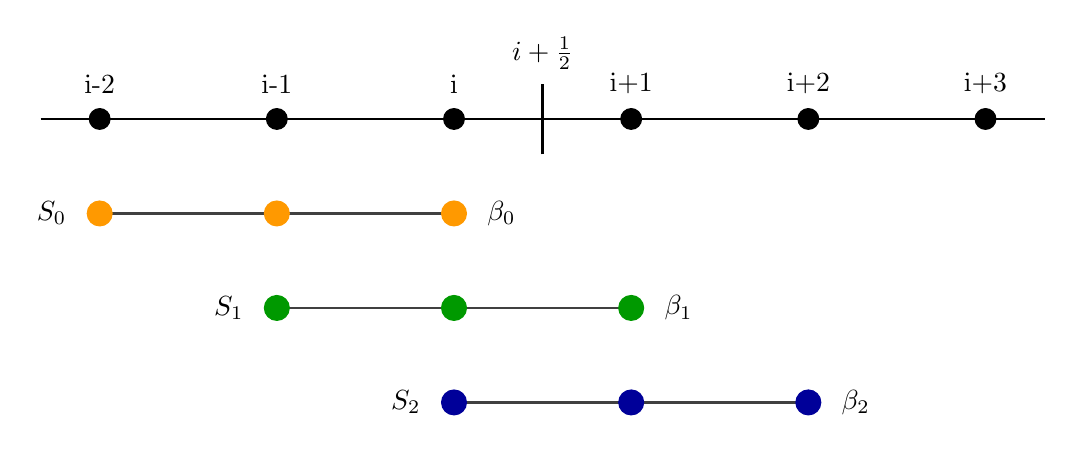
\begin{tikzpicture}[scale=1.5]
        % Draw horizontal line with equal extensions on both ends
        \draw[thick] (-3.5,0) -- (5,0);
        
        % Draw vertical line at i+1/2
        \draw[thick] (0.75,-0.3) -- (0.75,0.3);
        
        % Draw and label cell centres with equal spacing
        \foreach \x/\label in {-3/i-2, -1.5/i-1, 0/i, 1.5/i+1, 3/i+2, 4.5/i+3} {
            \filldraw[black] (\x,0) circle (2.5pt);
            \node[above=2mm] at (\x,0) {\label};
        }
        
        % Label i+1/2 positioned higher
        \node[above=5mm] at (0.75,0) {$i+\frac{1}{2}$};
        
        % Draw stencils with colors
        % S_2 (dark blue/navy)
        \draw[thick, darkgray] (0,-2.4) -- (3,-2.4);
        \foreach \x in {0, 1.5, 3} {
            \filldraw[blue!60!black] (\x,-2.4) circle (3pt);
        }
        \node[left=3mm] at (0,-2.4) {$S_2$};
        \node[right=3mm] at (3,-2.4) {$\beta_2$};
        
        % S_1 (green)
        \draw[thick, darkgray] (-1.5,-1.6) -- (1.5,-1.6);
        \foreach \x in {-1.5, 0, 1.5} {
            \filldraw[green!60!black] (\x,-1.6) circle (3pt);
        }
        \node[left=3mm] at (-1.5,-1.6) {$S_1$};
        \node[right=3mm] at (1.5,-1.6) {$\beta_1$};
        
        % S_0 (yellow/gold)
        \draw[thick, darkgray] (-3,-0.8) -- (0,-0.8);
        \foreach \x in {-3, -1.5, 0} {
            \filldraw[orange!80!yellow] (\x,-0.8) circle (3pt);
        }
        \node[left=3mm] at (-3,-0.8) {$S_0$};
        \node[right=3mm] at (0,-0.8) {$\beta_0$};
        
    \end{tikzpicture}
    \caption{Candidate stencils $S_0$, $S_1$, and $S_2$ for fifth-order WENO reconstruction at interface $i+\frac{1}{2}$~\citep{CastroEtAl2011}.}
    \label{figure:weno_stencil}
\end{figure}

% Considering an ENO reconstruction procedure that aims to approximate the solution at cell interfaces from cell-averaged or point values, a one-dimensional domain is discretised into cells of width $\Delta x$, where $x_i$ denotes the cell centre and $x_{i+1/2}$ denotes the interface between cells $i$ and $i+1$. For a given function $f(x)$, the ENO scheme constructs an $(r-1)$-th order polynomial approximation $S_r(x)$ on a stencil of $r$ points to interpolate the solution at the interface $x_{i+1/2}$. The stencil selection process begins with a base stencil and progressively adds points either to the left or right based on smoothness criteria. For each candidate stencil 
% \begin{equation}
% \mathcal{S}_k = \{x_{i-k}, x_{i-k+1}, \ldots, x_{i+r-k-1}\}
% \end{equation}
% with $k = 0, 1, \ldots, r-1$, a polynomial reconstruction $S_r^k(x)$ is computed such that $S_r^k(x_j) = f(x_j)$ for all $x_j \in \mathcal{S}_k$. The smoothness of each candidate reconstruction is quantified through an indicator, typically based on the sum of squared $L^2$ norms of all derivatives of $S_r^k(x)$ over the stencil. The stencil yielding the minimum smoothness indicator is selected, and the corresponding polynomial $S_r(x)$ is used to evaluate $f(x_{i+1/2}) \approx S_r(x_{i+1/2})$, providing the reconstructed value required for flux computation. For a scheme with $k$ candidate stencils spanning $2k-1$ cells, the reconstructed interface value can be expressed as
% \begin{equation}
% \hat{f}_{i+\frac{1}{2}}^{(r)} = \sum_{j=0}^{k-1} c_{rj} f_{i-r+j}, \quad r \in [0, k-1],
% \end{equation}
% where $c_{rj}$ are the ENO reconstruction coefficients. In standard ENO, only the single smoothest stencil is selected based on the minimum smoothness indicator, resulting in $k$-th order accuracy. In contrast, WENO schemes compute a weighted convex combination of all candidate stencils, where the weights are determined by the smoothness indicators. This weighted approach allows WENO to utilise information from all $2k-1$ cells in smooth regions, achieving $(2k-1)$-th order accuracy whilst maintaining the essentially non-oscillatory property near discontinuities.

% The smoothness indicators employed in WENO reconstruction play a critical role in determining the scheme's performance and accuracy. In the classical fifth-order WENO formulation by \citet{JiangShu1996}, smoothness indicators are constructed to measure the regularity of the solution on each candidate stencil, thereby guiding the weight distribution amongst the stencils. Whilst \citet{JiangShu1996} demonstrated that their scheme achieves the designed fifth-order accuracy in smooth regions, including at smooth extrema, subsequent analysis by \citet{HenrickEtAl2005} revealed potential accuracy degradation at certain types of critical points. To address this limitation, \citet{HenrickEtAl2005} introduced a mapped WENO (WENO-M) procedure that preserves the original smoothness indicator formulation but modifies the nonlinear weight computation through a mapping function, thereby restoring optimal order accuracy at critical points. It should be noted, however, that such accuracy degradation typically becomes significant only when the small parameter $\epsilon$ used to prevent division by zero is set to extremely small values (e.g., $\epsilon = 10^{-10}$ or smaller), which is rarely encountered in practical applications. Alternative improvements to the classical WENO framework include the WENO-Z scheme developed by \citet{BorgesEtAl2008} and further refined by \citet{CastroEtAl2011}, which incorporates a modified smoothness indicator that accounts for the relative smoothness across all candidate stencils, thereby enhancing the scheme's resolution properties in smooth regions whilst maintaining robust shock-capturing capabilities.


Considering an ENO reconstruction procedure that approximates the solution at cell interfaces from cell-averaged or point values, a one-dimensional domain is discretised into cells of width $\Delta x$, where $x_i$ denotes the cell centre and $x_{i+1/2}$ denotes the interface between cells $i$ and $i+1$. For a given function $f(x)$, the ENO scheme constructs an $(r-1)$-th order polynomial approximation $S_r(x)$ on a stencil of $r$ points to interpolate the solution at the interface $x_{i+1/2}$. The stencil selection process begins with a base stencil and progressively adds points either to the left or right based on smoothness criteria. For each candidate stencil 
\begin{equation}
\mathcal{S}_k = \{x_{i-k}, x_{i-k+1}, \ldots, x_{i+r-k-1}\}
\end{equation}
with $k = 0, 1, \ldots, r-1$, a polynomial reconstruction $S_r^k(x)$ is computed such that $S_r^k(x_j) = f(x_j)$ for all $x_j \in \mathcal{S}_k$. The smoothness of each candidate reconstruction is quantified through a smoothness indicator $\beta_k$, typically based on the sum of squared $L^2$ norms of all derivatives of $S_r^k(x)$ over the stencil. The stencil yielding the minimum smoothness indicator is selected, and the corresponding polynomial $S_r(x)$ is used to evaluate $f(x_{i+1/2}) \approx S_r(x_{i+1/2})$, providing the reconstructed value required for flux computation. 

For a scheme with $k$ candidate stencils spanning $2k-1$ cells, as illustrated in Figure~\ref{figure:weno_stencil} for the fifth-order case, the reconstructed interface value can be expressed as
\begin{equation}
\hat{f}_{i+\frac{1}{2}}^{(r)} = \sum_{j=0}^{k-1} c_{rj} f_{i-r+j}, \quad r \in [0, k-1],
\end{equation}
where $c_{rj}$ are the ENO reconstruction coefficients. In standard ENO, only the single smoothest stencil is selected based on the minimum smoothness indicator, resulting in $k$-th order accuracy. In contrast, WENO schemes compute a weighted convex combination of all candidate stencils, where the weights are determined by the smoothness indicators $\beta_k$. This weighted approach allows WENO to utilise information from all $2k-1$ cells in smooth regions, achieving $(2k-1)$-th order accuracy whilst maintaining the essentially non-oscillatory property near discontinuities.

The construction and properties of smoothness indicators are crucial to WENO performance and accuracy. In the classical fifth-order WENO formulation by \citet{JiangShu1996}, smoothness indicators measure the regularity of the solution on each candidate stencil, guiding the weight distribution amongst stencils. Whilst this scheme achieves fifth-order accuracy in smooth regions, \citet{HenrickEtAl2005} identified potential accuracy degradation at certain critical points and introduced a mapped WENO procedure to address this limitation. However, such degradation typically occurs only with extremely small values of the parameter $\epsilon$ (e.g., $\epsilon = 10^{-10}$), which are rarely used in practice. An important improvement to the classical WENO framework is the WENO-Z scheme developed by \citet{BorgesEtAl2008} and further refined by \citet{CastroEtAl2011}. WENO-Z incorporates a modified smoothness indicator that accounts for the relative smoothness across all candidate stencils, thereby enhancing the scheme's resolution properties in smooth regions whilst maintaining robust shock-capturing capabilities. This approach provides better discrimination between smooth and non-smooth stencils, leading to reduced numerical dissipation compared to the classical WENO formulation.

The formulation of smoothness indicators is fundamental to the WENO weighting strategy and directly impacts the scheme's ability to distinguish between smooth and discontinuous regions. In one dimension, the smoothness indicators quantify the local regularity of the solution by measuring the variation of the reconstructed polynomial and its derivatives over each candidate stencil. Following the framework established by \citet{JiangShu1996}, the smoothness indicator $\beta_k$ for each candidate stencil $S_k$ is defined as the weighted sum of $L^2$ norms of the derivatives of the interpolating polynomial $g_k(x)$ over the stencil interval:
\begin{equation}
\beta_k = \sum_{l=1}^{r-1} \int_{x_{i-\frac{1}{2}}}^{x_{i+\frac{1}{2}}} \Delta x^{2l-1} \left( \frac{\partial^l g_k}{\partial x^l} \right)^2 \mathrm{d}x,
\end{equation}
where $g_k(x)$ represents the $(r-1)$-th order interpolating polynomial constructed on stencil $S_k$. This formulation ensures that stencils crossing discontinuities yield significantly larger values of $\beta_k$ compared to those in smooth regions. For the fifth-order WENO scheme ($k=3$), the explicit expressions for the smoothness indicators on the three candidate stencils are:
\begin{align}
\beta_0 &= \frac{13}{12}(f_i - 2f_{i+1} + f_{i+2})^2 + \frac{1}{4}(3f_i - 4f_{i+1} + f_{i+2})^2, \\
\beta_1 &= \frac{13}{12}(f_{i-1} - 2f_i + f_{i+1})^2 + \frac{1}{4}(f_{i-1} - f_{i+1})^2, \\
\beta_2 &= \frac{13}{12}(f_{i-2} - 2f_{i-1} + f_i)^2 + \frac{1}{4}(f_{i-2} - 4f_{i-1} + 3f_i)^2.
\end{align}
The nonlinear weights are then computed as
\begin{equation}
\omega_k = \frac{\alpha_k}{\sum_{n=0}^{k-1} \alpha_n}, \quad \alpha_k = \frac{d_k}{(\epsilon + \beta_k)^p},
\end{equation}
where $d_k$ are the optimal linear weights, $\epsilon$ is a small parameter (typically $\epsilon = 10^{-6}$) to prevent division by zero, and $p$ is typically set to 2. For the fifth-order scheme, the optimal weights are $d_0 = 3/10$, $d_1 = 3/5$, and $d_2 = 1/10$.

The WENO-Z scheme modifies this formulation by introducing a global smoothness measure $\tau$ that captures higher-order information across the entire stencil. For the fifth-order case, this is defined as
\begin{equation}
\tau = |\beta_0 - \beta_2|,
\end{equation}
representing the absolute difference between the smoothness indicators of the outermost stencils. The modified nonlinear weights are then computed as
\begin{equation}
\omega_k^z = \frac{\alpha_k^z}{\sum_{n=0}^{2} \alpha_n^z}, \quad \alpha_k^z = d_k \left(1 + \left(\frac{\tau}{\epsilon + \beta_k}\right)^2\right),
\end{equation}
where the quadratic dependence on the ratio $\tau/(\epsilon + \beta_k)$ provides enhanced discrimination between smooth and discontinuous stencils compared to the classical JS formulation.

% Considering an ENO reconstruction procedure that aims to approximate the solution at cell interfaces from cell-averaged or point values, a one-dimensional domain is discretised into cells of width $\Delta x$, where $x_i$ denotes the cell centre and $x_{i+1/2}$ denotes the interface between cells $i$ and $i+1$. For a given function $f(x)$, the ENO scheme constructs an $(r-1)$-th order polynomial approximation $S_r(x)$ on a stencil of $r$ points to interpolate the solution at the interface $x_{i+1/2}$. The stencil selection process begins with a base stencil and progressively adds points either to the left or right based on smoothness criteria. For each candidate stencil 
% \begin{equation}
% \mathcal{S}_k = \{x_{i-k}, x_{i-k+1}, \ldots, x_{i+r-k-1}\}
% \end{equation}
% with $k = 0, 1, \ldots, r-1$, a polynomial reconstruction $S_r^k(x)$ is computed such that $S_r^k(x_j) = f(x_j)$ for all $x_j \in \mathcal{S}_k$. The smoothness of each candidate reconstruction is quantified through an indicator, typically based on the sum of squared $L^2$ norms of all derivatives of $S_r^k(x)$ over the stencil. The stencil yielding the minimum smoothness indicator is selected, and the corresponding polynomial $S_r(x)$ is used to evaluate $f(x_{i+1/2}) \approx S_r(x_{i+1/2})$, providing the reconstructed value required for flux computation. For a scheme with $k$ candidate stencils spanning $2k-1$ cells, the reconstructed interface value can be expressed as
% \begin{equation}
% \hat{f}_{i+\frac{1}{2}}^{(r)} = \sum_{j=0}^{k-1} c_{rj} f_{i-r+j}, \quad r \in [0, k-1],
% \end{equation}
% where $c_{rj}$ are the ENO reconstruction coefficients. In standard ENO, only the single smoothest stencil is selected based on the minimum smoothness indicator, resulting in $k$-th order accuracy. In contrast, WENO schemes compute a weighted convex combination of all candidate stencils, where the weights are determined by the smoothness indicators. This weighted approach allows WENO to utilise information from all $2k-1$ cells in smooth regions, achieving $(2k-1)$-th order accuracy whilst maintaining the essentially non-oscillatory property near discontinuities.

% The construction and properties of smoothness indicators are crucial to WENO performance and accuracy. In the classical fifth-order WENO formulation by \citet{JiangShu1996}, smoothness indicators measure the regularity of the solution on each candidate stencil, guiding the weight distribution amongst stencils. Whilst this scheme achieves fifth-order accuracy in smooth regions, \citet{HenrickEtAl2005} identified potential accuracy degradation at certain critical points and introduced a mapped WENO procedure to address this limitation. However, such degradation typically occurs only with extremely small values of the parameter $\epsilon$ (e.g., $\epsilon = 10^{-10}$), which are rarely used in practice. An important improvement to the classical WENO framework is the WENO-Z scheme developed by \citet{BorgesEtAl2008} and further refined by \citet{CastroEtAl2011}. WENO-Z incorporates a modified smoothness indicator that accounts for the relative smoothness across all candidate stencils, thereby enhancing the scheme's resolution properties in smooth regions whilst maintaining robust shock-capturing capabilities. This approach provides better discrimination between smooth and non-smooth stencils, leading to reduced numerical dissipation compared to the classical WENO formulation.

% The construction and properties of smoothness indicators are crucial to WENO performance and accuracy. In the classical fifth-order WENO formulation by \citet{JiangShu1996}, smoothness indicators are constructed to measure the regularity of the solution on each candidate stencil, thereby guiding the weight distribution amongst the stencils. Whilst \citet{JiangShu1996} demonstrated that their scheme achieves the designed fifth-order accuracy in smooth regions, including at smooth extrema, subsequent analysis by \citet{HenrickEtAl2005} revealed potential accuracy degradation at certain types of critical points. To address this limitation, \citet{HenrickEtAl2005} introduced a mapped WENO (WENO-M) procedure that preserves the original smoothness indicator formulation but modifies the nonlinear weight computation through a mapping function, thereby restoring optimal order accuracy at critical points. It should be noted, however, that such accuracy degradation typically becomes significant only when the small parameter $\epsilon$ used to prevent division by zero is set to extremely small values (e.g., $\epsilon = 10^{-10}$ or smaller), which is rarely encountered in practical applications. Alternative improvements to the classical WENO framework include the WENO-Z scheme developed by \citet{BorgesEtAl2008} and further refined by \citet{CastroEtAl2011}, which incorporates a modified smoothness indicator that accounts for the relative smoothness across all candidate stencils, thereby enhancing the scheme's resolution properties in smooth regions whilst maintaining robust shock-capturing capabilities.


% More recently, Targeted ENO (TENO) schemes \citep{FuEtAl2016,FuEtAl2017} utilise a scale-separation procedure combined with candidate stencils of varying width to achieve lower numerical dissipation compared to classical WENO schemes whilst preserving sharp shock-capturing capability for discontinuities.



% Considering an ENO reconstruction procedure that aims to approximate the solution at cell interfaces from cell-averaged or point values, a one-dimensional domain is discretised into cells of uniform width $\Delta x$, where $x_i$ denotes the cell centre and $x_{i+1/2}$ denotes the interface between cells $i$ and $i+1$. For a given function $f(x)$, the ENO scheme constructs an $(r-1)$-th order polynomial approximation $S_r(x)$ on a stencil of $r$ points to interpolate the solution at the interface $x_{i+1/2}$. The stencil selection process begins with a base stencil and progressively adds points either to the left or right based on smoothness criteria, ensuring that the chosen stencil avoids crossing discontinuities wherever possible. For each candidate stencil 
% \begin{equation}
% \mathcal{S}_k = \{x_{i-k}, x_{i-k+1}, \ldots, x_{i+r-k-1}\}
% \end{equation}
% with $k = 0, 1, \ldots, r-1$, a polynomial reconstruction $S_r^k(x)$ is computed such that $S_r^k(x_j) = f(x_j)$ for all $x_j \in \mathcal{S}_k$. The smoothness of each candidate reconstruction is quantified through a smoothness indicator, typically based on the sum of squared $L^2$ norms of all derivatives of $S_r^k(x)$ over the stencil interval. The stencil yielding the minimum smoothness indicator is selected, and the corresponding polynomial $S_r(x)$ is then used to evaluate $f(x_{i+1/2}) \approx S_r(x_{i+1/2})$, providing the reconstructed value required for flux computation. For a scheme with $k$ candidate stencils spanning $2k-1$ cells, the reconstructed interface value can be expressed as
% \begin{equation}
% \hat{f}_{i+\frac{1}{2}}^{(r)} = \sum_{j=0}^{k-1} c_{rj} f_{i-r+j}, \quad r \in [0, k-1],
% \end{equation}
% where $c_{rj}$ are the ENO reconstruction coefficients that depend on the chosen stencil configuration. In standard ENO, only the single smoothest stencil is selected based on the minimum smoothness indicator, resulting in $k$-th order accuracy in smooth regions. In contrast, WENO schemes compute a weighted convex combination of all candidate stencils, where the weights are determined by the smoothness indicators of each stencil. This weighted approach allows WENO to effectively utilise information from all $2k-1$ cells in smooth regions, achieving $(2k-1)$-th order accuracy whilst maintaining the essentially non-oscillatory property near discontinuities.




\subsubsection{Characteristic decomposition}

For systems of hyperbolic conservation laws, applying WENO reconstruction directly to the conserved variables can lead to spurious oscillations near discontinuities, particularly when different characteristic waves interact. To address this, the WENO reconstruction is performed in characteristic space rather than physical space, following the approach outlined by \citet{JiangShu1996}. The characteristic decomposition transforms the system of equations into decoupled scalar advection equations along each characteristic direction, allowing the WENO scheme to treat each wave independently. Consider a system of conservation laws $\mathbf{U}_t + \mathbf{F}(\mathbf{U})_x = 0$, where $\mathbf{U}$ is the vector of conserved variables and $\mathbf{F}(\mathbf{U})$ is the flux vector. The Jacobian matrix $\mathbf{A} = \partial \mathbf{F}/\partial \mathbf{U}$ can be diagonalised using its left and right eigenvector matrices, $\mathbf{R}^{-1}$ and $\mathbf{R}$ respectively, such that
\begin{equation}
\mathbf{W} = \mathbf{R}^{-1}\mathbf{U},
\end{equation}
transforms the hyperbolic system into diagonal form
\begin{equation}
\mathbf{W}_t + \mathbf{\Lambda}\mathbf{W}_x = 0,
\end{equation}
where $\mathbf{\Lambda}$ is the diagonal matrix of eigenvalues $\lambda_j$ corresponding to the characteristic speeds. The WENO reconstruction is then applied to each component of the characteristic variable vector $\mathbf{V}$, treating each as an independent scalar equation. Following reconstruction in characteristic space, the solution is transformed back to physical space through
\begin{equation}
\mathbf{U} = \mathbf{R}\mathbf{W}.
\end{equation}
For systems with variable coefficients, such as the reactive Navier-Stokes equations where thermochemical properties vary spatially, the matrices $\mathbf{R}$, $\mathbf{R}^{-1}$, and $\mathbf{\Lambda}$ depend on the local state $\mathbf{U}$ and must be evaluated at each cell interface. A common approach is to use a locally averaged state at the interface $\mathbf{U}_{i+\frac{1}{2}}$, with the arithmetic mean $\mathbf{U}_{i+\frac{1}{2}} = (\mathbf{U}_i + \mathbf{U}_{i+1})/2$ being the simplest choice, though more sophisticated averages such as the Roe average can provide improved accuracy.

\subsubsection{Flux Jacobian and eigenvectors}

High-order shock-capturing schemes applied to thermochemically reacting flows necessitate accurate eigendecomposition of the flux Jacobian to facilitate characteristic-based reconstruction. The development of such formulations for high-enthalpy flows traces back to \citet{Gnoffo1989}, with subsequent extensions by \citet{GrossmanCinnella1990} and \citet{ShuenEtAl1990} addressing chemical and vibrational nonequilibrium effects. The Roe-averaging framework of \citet{GrossmanCinnella1990} incorporated species-specific vibrational temperatures through harmonic oscillator models, whilst \citet{ShuenEtAl1990} introduced a pressure-correction methodology to maintain thermodynamic consistency of the averaged state for chemically reacting flows in vibrational equilibrium. Extension to generalised curvilinear coordinates for multi-temperature reactive systems was achieved by \citet{WangZhong2009}. The Jacobian eigendecomposition employed in this study follows the formulation for thermochemical nonequilibrium in Cartesian coordinates.

% For the thermally non-equilibrium and chemically reacting \gls{TCNE} system in the $x$-direction, the inviscid flux Jacobian is defined as
% \begin{equation}
% \mathbf{A} = \frac{\partial \mathbf{F}}{\partial \mathbf{U}} = \mathbf{L}\mathbf{\Lambda}\mathbf{R},
% \end{equation}
% where the inviscid flux vector $\mathbf{F}$ in the $x$-direction is
% \begin{equation}
% \mathbf{F} = \begin{bmatrix}
% \rho_1 u \\
% \rho_2 u \\
% \vdots \\
% \rho_{N_s} u \\
% \rho u^2 + p \\
% \rho uv \\
% \rho uw \\
% \rho u H \\
% \rho e_v u
% \end{bmatrix}.
% \end{equation}
% where the right eigenvector matrix $\mathbf{R}$ is given by
% \begin{equation}
% \mathbf{R} = \begin{bmatrix}
% a^2\delta_{sr} - Y_s\gamma_{f,r} & \beta u Y_s & \beta v Y_s & \beta w Y_s & -\beta Y_s & -\phi Y_s \\
% -\mathcal{V} & l_x & l_y & l_z & 0 & 0 \\
% -\mathcal{W} & m_x & m_y & m_z & 0 & 0 \\
% \gamma_{f,r} - \mathcal{U}a & a n_x - \beta u & a n_y - \beta v & a n_z - \beta w & \beta & \phi \\
% \gamma_{f,r} + \mathcal{U}a & -a n_x - \beta u & -a n_y - \beta v & -a n_z - \beta w & \beta & \phi \\
% -e_v\gamma_{f,r} & \beta u e_v & \beta v e_v & \beta w e_v & -\beta e_v & a^2 - \phi e_v
% \end{bmatrix}
% \end{equation}
% and the left eigenvector matrix $\mathbf{L}$ is
% \begin{equation}
% \mathbf{L} = \begin{bmatrix}
% \delta_{sr}/a^2 & 0 & 0 & Y_s/(2a^2) & Y_s/(2a^2) & 0 \\
% u/a^2 & l_x & m_x & (u+a n_x)/(2a^2) & (u-a n_x)/(2a^2) & 0 \\
% v/a^2 & l_y & m_y & (v+a n_y)/(2a^2) & (v-a n_y)/(2a^2) & 0 \\
% w/a^2 & l_z & m_z & (w+a n_z)/(2a^2) & (w-a n_z)/(2a^2) & 0 \\
% G_r/a^2 & \mathcal{V} & \mathcal{W} & (H+a\mathcal{U})/(2a^2) & (H-a\mathcal{U})/(2a^2) & -\phi/\beta a^2 \\
% 0 & 0 & 0 & e_v/(2a^2) & e_v/(2a^2) & 1/a^2
% \end{bmatrix}
% \end{equation}
% The diagonal eigenvalue matrix $\mathbf{\Lambda}$ contains the characteristic speeds
% \begin{align}
% \lambda_{1,2,3,4,5,6,7,\ldots,N_s+4} &= u, \\
% \lambda_{N_s+5} &= u + a, \\
% \lambda_{N_s+6} &= u - a,
% \end{align}
% where $\mathbf{n} = (n_x, n_y, n_z) = (k_1, k_2, k_3)/|\mathbf{k}|$ is the unit normal vector, $\mathbf{l} = (l_x, l_y, l_z)$ and $\mathbf{m} = (m_x, m_y, m_z)$ are two unit vectors orthogonal to $\mathbf{n}$ and to each other, and
% \begin{align}
% \mathcal{U} &= un_x + vn_y + wn_z, \\
% \mathcal{V} &= ul_x + vl_y + wl_z, \\
% \mathcal{W} &= um_x + vm_y + wm_z.
% \end{align}
% The thermochemical parameters appearing in the Jacobian matrices are defined as
% \begin{align}
% G_r &= \beta(u^2+v^2+w^2) - \gamma_{f,r}, \\[0.8em]
% \beta &= \frac{\mathcal{R}}{\rho}\sum_{s=1}^{N_s}\frac{\rho_s}{M_s}, \\[0.8em]
% \phi &= -\beta, \\[0.8em]
% \gamma_{f,r} &= \frac{\mathcal{R}T}{M_s} + \beta\frac{u^2+v^2+w^2}{2} - \beta e_s - \phi e_{v,s}, \\[0.8em]
% a^2 &= \sum_{s=1}^{N_s}Y_s\gamma_{f,s} + \beta\left[H - (u^2+v^2+w^2)\right] + \phi e_v,
% \end{align}
% where $a$ is the frozen speed of sound, and the subscripts $s$ and $r$ denote species and spatial indices respectively. It should be noted that the above Jacobian formulation applies to flows in chemical nonequilibrium or chemically frozen conditions, where the frozen speed of sound $a$ is appropriate. Flows approaching chemical equilibrium require a modified treatment to incorporate the equilibrium speed of sound, as presented by \citet{LiouEtAl1990}. Considering flows in vibrational equilibrium, 


For the thermally non-equilibrium and chemically reacting \gls{TCNE} system in the direction $\mathbf{n} = (n_x, n_y, n_z)$, the inviscid flux Jacobian is defined as
\begin{equation}
\mathbf{A} = \frac{\partial \mathbf{F}}{\partial \mathbf{U}} = \mathbf{L}\mathbf{\Lambda}\mathbf{R},
\end{equation}
where the inviscid flux vector $\mathbf{F}$ in the $\mathbf{n}$-direction is
\begin{equation}
\mathbf{F} = \begin{bmatrix}
\rho_1 \mathbf{n} \cdot \mathbf{u} \\
\rho_2 \mathbf{n} \cdot \mathbf{u} \\
\vdots \\
\rho_{N_s} \mathbf{n} \cdot \mathbf{u} \\
\rho u \mathbf{n} \cdot \mathbf{u} + p n_x \\
\rho v \mathbf{n} \cdot \mathbf{u} + p n_y \\
\rho w \mathbf{n} \cdot \mathbf{u} + p n_z \\
\rho H \mathbf{n} \cdot \mathbf{u} \\
\rho e_v \mathbf{n} \cdot \mathbf{u}
\end{bmatrix},
\end{equation}
where $\mathbf{u} = (u, v, w)$ is the velocity vector and $\mathbf{n} \cdot \mathbf{u} = un_x + vn_y + wn_z$ is the contravariant velocity. The right eigenvector matrix $\mathbf{R}$ is given by
\begin{equation}
\mathbf{R} = \begin{bmatrix}
a^2\delta_{sr} - Y_s\gamma_{f,r} & \beta u Y_s & \beta v Y_s & \beta w Y_s & -\beta Y_s & -\phi Y_s \\
-\mathcal{V} & l_x & l_y & l_z & 0 & 0 \\
-\mathcal{W} & m_x & m_y & m_z & 0 & 0 \\
\gamma_{f,r} - \mathcal{U}a & a n_x - \beta u & a n_y - \beta v & a n_z - \beta w & \beta & \phi \\
\gamma_{f,r} + \mathcal{U}a & -a n_x - \beta u & -a n_y - \beta v & -a n_z - \beta w & \beta & \phi \\
-e_v\gamma_{f,r} & \beta u e_v & \beta v e_v & \beta w e_v & -\beta e_v & a^2 - \phi e_v
\end{bmatrix}
\end{equation}
and the left eigenvector matrix $\mathbf{L}$ is
\begin{equation}
\mathbf{L} = \begin{bmatrix}
\delta_{sr}/a^2 & 0 & 0 & Y_s/(2a^2) & Y_s/(2a^2) & 0 \\
u/a^2 & l_x & m_x & (u+a n_x)/(2a^2) & (u-a n_x)/(2a^2) & 0 \\
v/a^2 & l_y & m_y & (v+a n_y)/(2a^2) & (v-a n_y)/(2a^2) & 0 \\
w/a^2 & l_z & m_z & (w+a n_z)/(2a^2) & (w-a n_z)/(2a^2) & 0 \\
G_r/a^2 & \mathcal{V} & \mathcal{W} & (H+a\mathcal{U})/(2a^2) & (H-a\mathcal{U})/(2a^2) & -\phi/\beta a^2 \\
0 & 0 & 0 & e_v/(2a^2) & e_v/(2a^2) & 1/a^2
\end{bmatrix}.
\end{equation}
The diagonal eigenvalue matrix $\mathbf{\Lambda}$ contains the characteristic speeds
\begin{equation}
\lambda_{1,\ldots,N_s+4} = \mathbf{n} \cdot \mathbf{u}, \quad \lambda_{N_s+5} = \mathbf{n} \cdot \mathbf{u} + a, \quad \lambda_{N_s+6} = \mathbf{n} \cdot \mathbf{u} - a,
\end{equation}
where $\mathbf{n} = (n_x, n_y, n_z)$ is the unit normal vector in the computational coordinate direction, $\mathbf{l} = (l_x, l_y, l_z)$ and $\mathbf{m} = (m_x, m_y, m_z)$ are two unit vectors orthogonal to $\mathbf{n}$ and to each other, and
\begin{align}
\mathcal{U} &= un_x + vn_y + wn_z = \mathbf{n} \cdot \mathbf{u}, \\
\mathcal{V} &= ul_x + vl_y + wl_z = \mathbf{l} \cdot \mathbf{u}, \\
\mathcal{W} &= um_x + vm_y + wm_z = \mathbf{m} \cdot \mathbf{u}.
\end{align}
The thermochemical parameters appearing in the Jacobian matrices are defined as
\begin{align}
G_r &= \beta(u^2+v^2+w^2) - \gamma_{f,r}, \\[0.8em]
\beta &= \frac{\mathcal{R}}{\rho}\sum_{s=1}^{N_s}\frac{\rho_s}{M_s}, \\[0.8em]
\phi &= -\beta, \\[0.8em]
\gamma_{f,r} &= \frac{\mathcal{R}T}{M_s} + \beta\frac{u^2+v^2+w^2}{2} - \beta e_s - \phi e_{v,s}, \\[0.8em]
a^2 &= \sum_{s=1}^{N_s}Y_s\gamma_{f,s} + \beta\left[H - (u^2+v^2+w^2)\right] + \phi e_v,
\end{align}
where $a$ is the frozen speed of sound. For non-ionised flows, the frozen speed of sound reduces to
\begin{equation}
a^2 = (1 + \beta)\frac{p}{\rho}
\end{equation}
which recovers the classical expression for calorically perfect gases when $\beta = \gamma - 1$. The subscripts $s$ and $r$ denote species and spatial indices respectively.

It should be noted that the above Jacobian formulation applies to flows in chemical nonequilibrium or chemically frozen conditions, where the frozen speed of sound $a$ is appropriate. Flows approaching chemical equilibrium require a modified treatment to incorporate the equilibrium speed of sound, as presented by \citet{LiouEtAl1990}. 

For chemically reacting flows in thermodynamic equilibrium (\gls{TEQ}) and \gls{CPG} flows, the inviscid flux Jacobian in the direction $\mathbf{n} = (n_x, n_y, n_z)$ is defined as
\begin{equation}
\mathbf{A} = \frac{\partial \mathbf{F}}{\partial \mathbf{U}} = \mathbf{L}\mathbf{\Lambda}\mathbf{R},
\end{equation}
where the inviscid flux vector $\mathbf{F}$ in the $\mathbf{n}$-direction is
\begin{equation}
\mathbf{F} = \begin{bmatrix}
\rho_1 \mathbf{n} \cdot \mathbf{u} \\
\rho_2 \mathbf{n} \cdot \mathbf{u} \\
\vdots \\
\rho_{N_s} \mathbf{n} \cdot \mathbf{u} \\
\rho u \mathbf{n} \cdot \mathbf{u} + p n_x \\
\rho v \mathbf{n} \cdot \mathbf{u} + p n_y \\
\rho w \mathbf{n} \cdot \mathbf{u} + p n_z \\
\rho H \mathbf{n} \cdot \mathbf{u}
\end{bmatrix}.
\end{equation}
The flux vector structure is identical for both \gls{TEQ} and \gls{CPG} cases, with the distinction arising in the total enthalpy $H$, which includes vibrational energy contributions in \gls{TEQ} flows but excludes them in \gls{CPG} flows where vibrational modes are not excited. 

The right eigenvector matrix $\mathbf{R}$ is given by
\begin{equation}
\mathbf{R} = \begin{bmatrix}
a_{eq}^2\delta_{sr} - Y_s\gamma_{eq,r} & \beta_{eq} u Y_s & \beta_{eq} v Y_s & \beta_{eq} w Y_s & -\beta_{eq} Y_s \\
-\mathcal{V} & l_x & l_y & l_z & 0 \\
-\mathcal{W} & m_x & m_y & m_z & 0 \\
\gamma_{eq,r} - \mathcal{U}a_{eq} & a_{eq} n_x - \beta_{eq} u & a_{eq} n_y - \beta_{eq} v & a_{eq} n_z - \beta_{eq} w & \beta_{eq} \\
\gamma_{eq,r} + \mathcal{U}a_{eq} & -a_{eq} n_x - \beta_{eq} u & -a_{eq} n_y - \beta_{eq} v & -a_{eq} n_z - \beta_{eq} w & \beta_{eq}
\end{bmatrix}
\end{equation}
and the left eigenvector matrix $\mathbf{L}$ is
\begin{equation}
\mathbf{L} = \begin{bmatrix}
\delta_{sr}/a_{eq}^2 & 0 & 0 & Y_s/(2a_{eq}^2) & Y_s/(2a_{eq}^2) \\
u/a_{eq}^2 & l_x & m_x & (u+a_{eq} n_x)/(2a_{eq}^2) & (u-a_{eq} n_x)/(2a_{eq}^2) \\
v/a_{eq}^2 & l_y & m_y & (v+a_{eq} n_y)/(2a_{eq}^2) & (v-a_{eq} n_y)/(2a_{eq}^2) \\
w/a_{eq}^2 & l_z & m_z & (w+a_{eq} n_z)/(2a_{eq}^2) & (w-a_{eq} n_z)/(2a_{eq}^2) \\
G_{eq,r}/a_{eq}^2 & \mathcal{V} & \mathcal{W} & (H+a_{eq}\mathcal{U})/(2a_{eq}^2) & (H-a_{eq}\mathcal{U})/(2a_{eq}^2)
\end{bmatrix}.
\end{equation}
The diagonal eigenvalue matrix $\mathbf{\Lambda}$ contains the characteristic speeds
\begin{equation}
\lambda_{1,\ldots,N_s+3} = \mathbf{n} \cdot \mathbf{u}, \quad \lambda_{N_s+4} = \mathbf{n} \cdot \mathbf{u} + a_{eq}, \quad \lambda_{N_s+5} = \mathbf{n} \cdot \mathbf{u} - a_{eq},
\end{equation}

The thermochemical parameters for equilibrium flows are defined as
\begin{align}
G_{eq,r} &= \beta_{eq}(u^2+v^2+w^2) - \gamma_{eq,r}, \\[0.8em]
\beta_{eq} &= \frac{\mathcal{R}}{\rho}\sum_{s=1}^{N_s}\frac{\rho_s}{M_s} + \left(\frac{\partial p}{\partial E}\right)_{\rho,\rho_s}, \\[0.8em]
\gamma_{eq,r} &= \frac{\mathcal{R}T}{M_s} + \beta_{eq}\frac{u^2+v^2+w^2}{2} - \beta_{eq} e_s, \\[0.8em]
a_{eq}^2 &= \sum_{s=1}^{N_s}Y_s\gamma_{eq,s} + \beta_{eq}\left[H - (u^2+v^2+w^2)\right],
\end{align}
where $a_{eq}$ is the equilibrium speed of sound, which accounts for thermochemical relaxation effects through the modified parameter $\beta_{eq}$ \citep{LiouEtAl1990}.



% For the thermally non-equilibrium and chemically reacting system in the $x$-direction, the inviscid flux Jacobian is defined as
% \begin{equation}
% \mathbf{A} = \frac{\partial \mathbf{F}}{\partial \mathbf{U}} = \mathbf{L}\mathbf{\Lambda}\mathbf{R},
% \end{equation}
% where the right eigenvector matrix $\mathbf{R}$ is given by
% \begin{equation}
% \mathbf{R} = \begin{bmatrix}
% a^2\delta_{sr} - c_s\tilde{\gamma}_r & \beta u c_s & \beta v c_s & \beta w c_s & -\beta c_s & -\phi c_s \\
% -\tilde{V} & l_x & l_y & l_z & 0 & 0 \\
% -\tilde{W} & m_x & m_y & m_z & 0 & 0 \\
% \tilde{\gamma}_r - \tilde{U}a & an_x - \beta u & an_y - \beta v & an_z - \beta w & \beta & \phi \\
% \tilde{\gamma}_r + \tilde{U}a & -an_x - \beta u & -an_y - \beta v & -an_z - \beta w & \beta & \phi \\
% -e_V\tilde{\gamma}_r & \beta u e_V & \beta v e_V & \beta w e_V & -\beta e_V & a^2 - \phi e_V
% \end{bmatrix},
% \end{equation}
% and the left eigenvector matrix $\mathbf{L}$ is
% \begin{equation}
% \mathbf{L} = \begin{bmatrix}
% \delta_{sr}/a^2 & 0 & 0 & c_s/(2a^2) & c_s/(2a^2) & 0 \\
% u/a^2 & l_x & m_x & (u+an_x)/(2a^2) & (u-an_x)/(2a^2) & 0 \\
% v/a^2 & l_y & m_y & (v+an_y)/(2a^2) & (v-an_y)/(2a^2) & 0 \\
% w/a^2 & l_z & m_z & (w+an_z)/(2a^2) & (w-an_z)/(2a^2) & 0 \\
% G_r/a^2 & \tilde{V} & \tilde{W} & (H+a\tilde{U})/(2a^2) & (H-a\tilde{U})/(2a^2) & -\phi/\beta a^2 \\
% 0 & 0 & 0 & e_V/(2a^2) & e_V/(2a^2) & 1/a^2
% \end{bmatrix}.
% \end{equation}
% The diagonal eigenvalue matrix $\mathbf{\Lambda}$ contains the characteristic speeds
% \begin{align}
% \lambda_{1,2,3,4,5,6,7,\ldots,N_s+4} &= u, \\
% \lambda_{N_s+5} &= u + a, \\
% \lambda_{N_s+6} &= u - a,
% \end{align}
% where $\mathbf{n} = (n_x, n_y, n_z) = (k_1, k_2, k_3)/|\mathbf{k}|$ is the unit normal vector, $\mathbf{l} = (l_x, l_y, l_z)$ and $\mathbf{m} = (m_x, m_y, m_z)$ are two unit vectors orthogonal to $\mathbf{n}$ and to each other, and
% \begin{align}
% \tilde{U} &= un_x + vn_y + wn_z, \\
% \tilde{V} &= ul_x + vl_y + wl_z, \\
% \tilde{W} &= um_x + vm_y + wm_z.
% \end{align}
% The thermochemical parameters appearing in the Jacobian matrices are defined as
% \begin{align}
% G_r &= \beta(u^2+v^2+w^2) - \tilde{\gamma}_r, \\[0.8em]
% \beta &= \frac{\bar{R}}{\rho}\sum_{s=1}^{N_s}\frac{\rho_s}{M_s}, \\[0.8em]
% \phi &= -\beta, \\[0.8em]
% \tilde{\gamma}_r &= \frac{\bar{R}T}{M_s} + \beta\frac{u^2+v^2+w^2}{2} - \beta e_s - \phi e_{V,s}, \\[0.8em]
% a^2 &= \sum_{s=1}^{N_s}c_s\tilde{\gamma}_s + \beta\left[H - (u^2+v^2+w^2)\right] + \phi e_V,
% \end{align}
% where $a$ is the frozen speed of sound, and the subscripts $s$ and $r$ denote species and spatial indices respectively.

\subsubsection{Roe average}

The characteristic decomposition described above requires evaluation of the Jacobian matrices at cell interfaces, where the flow state is discontinuous. A common approach is to employ Roe averaging, which constructs an averaged state that satisfies certain consistency properties. The Roe-averaged state $\Psi(\mathbf{U})$ at interface $i+\frac{1}{2}$ must satisfy three conditions: (1) it should depend continuously on the left and right states $\mathbf{U}_L$ and $\mathbf{U}_R$, (2) it should reduce to the exact state when $\mathbf{U}_L = \mathbf{U}_R$, and (3) the resulting approximate Jacobian $\Psi(\mathbf{A})$ must satisfy the property
\begin{equation}
\Psi(\mathbf{A})(\mathbf{U}_R - \mathbf{U}_L) = \mathbf{F}_R - \mathbf{F}_L.
\end{equation}

For thermochemically reacting flows, the Roe-averaged primitive variables are computed using density-weighted averages. The Roe-averaging operator is defined as
\begin{equation}
\Psi(\mathcal{X}) = \frac{\sqrt{\rho_R}\mathcal{X}_R + \sqrt{\rho_L}\mathcal{X}_L}{\sqrt{\rho_R} + \sqrt{\rho_L}},
\end{equation}
where $\mathcal{X}$ represents any primitive variable. The Roe-averaged density is defined as
\begin{equation}
\Psi(\rho) = \sqrt{\rho_L \rho_R},
\end{equation}
and the Roe-averaged velocities and total enthalpy follow from the general operator:
\begin{equation}
\Psi(u) = \frac{\sqrt{\rho_L}u_L + \sqrt{\rho_R}u_R}{\sqrt{\rho_L} + \sqrt{\rho_R}}, \quad \Psi(H) = \frac{\sqrt{\rho_L}H_L + \sqrt{\rho_R}H_R}{\sqrt{\rho_L} + \sqrt{\rho_R}}.
\end{equation}
For flows in thermochemical nonequilibrium, the species densities and vibrational energy are averaged using arithmetic means:
\begin{equation}
\Psi(\rho_s) = \frac{\rho_{s,L} + \rho_{s,R}}{2}, \quad \Psi(e_v) = \frac{e_{v,L} + e_{v,R}}{2}.
\end{equation}
The thermochemical parameters $\beta$, $\phi$, $\gamma_{f,r}$, and the frozen or equilibrium speed of sound are then evaluated using the Roe-averaged state through the definitions provided in the previous section. These averaged quantities, including the contravariant velocities $\Psi(\mathcal{U})$, $\Psi(\mathcal{V})$, and $\Psi(\mathcal{W})$, are subsequently used to construct the eigenvector matrices $\mathbf{L}$ and $\mathbf{R}$ and the eigenvalue matrix $\mathbf{\Lambda}$ required for the characteristic decomposition.


\section{Boundary conditions}
The implementation of flows with vibrational nonequilibrium necessitates careful treatment of boundary conditions to ensure physical consistency and numerical stability. Particular attention must be given to the proper specification of vibrational energy at domain boundaries, alongside conventional thermodynamic and transport variables. 

% This section presents the boundary conditions employed in the present study, with emphasis on modifications required to accommodate vibrational excitation in thermochemical flows.

\subsection{Inflow conditions}
Compressible simulations of shock-wave boundary layer interactions require well-resolved inlet boundary layers. To avoid numerical instabilities at the inflow-wall interface caused by discontinuous flow profiles, an initial boundary layer is imposed into the computational domain rather than developing it from a sharp leading edge. This approach reduces computational cost and provides control over the target boundary layer thickness.

The boundary layer profiles are generated by solving the compressible Blasius equation through the Illingworth transformation \citep{White2005}. The differential equations detailed in Section~\ref{section:locallysimilar} are numerically integrated with specified freestream Mach number, freestream temperature, and Reynolds number based on the inlet displacement thickness $Re_{\delta^{*}_{0}}$. The resulting self-similar profiles provide the velocity $\mathrm{d}f/\mathrm{d}\eta$ and temperature $g(\eta)$ distributions in similarity coordinates, which are transformed to physical coordinates. The Reynolds number at a target location $x_d$ within the computational domain is computed as
\begin{equation}
    Re_x = \frac{1}{2} \left( \frac{Re_{\delta^{*}_0}}{\Delta_s} \right )^2 + x_d Re_{\delta^{*}_{0}}.
\end{equation}

For flows in thermochemical nonequilibrium, the inlet profiles include velocity components $(u, v)$, translational-rotational temperature $T$, vibrational temperature $T_v$, and species mass fractions $(Y_{\mathrm{N}_2}, Y_{\mathrm{O}_2}, \ldots)$. The implementation employs cubic spline interpolation based on \citet{numericalrecipies2007} to impose these profiles onto arbitrary computational grids, accommodating grid stretching through symbolic polynomial fits. The detailed formulation of the locally similar boundary layer equations and their extension to include vibrational excitation and chemical composition are presented in Section~\ref{section:locallysimilar}. 


\subsection{Numerical solution of similarity equations}\label{section:similaritysolution}

The similarity equation sets for thermochemical nonequilibrium flows are typically solved using shooting methods, wherein unknown wall values are estimated and the equations integrated outward to the freestream. An iterative scheme updates the wall estimates until freestream boundary conditions are satisfied. However, at high Mach numbers with wall cooling and chemical effects, convergence becomes sensitive to initial estimates, which can be difficult to construct accurately.

\begin{figure}[t]
    \centering
    \fontsize{9}{10}\selectfont
    \includegraphics[width=0.5\textwidth]{resources/figures/opensbli/result_ssprofiles_literature.pdf}
    \caption{Validation of self-similar boundary layer profiles against DNS and literature data. Normalised velocity $f'$ and temperature $\theta$ profiles in similarity coordinates for Mach 10 flow in thermal equilibrium with a non-catalytic adiabatic wall.}
    \label{figure:similarity_validation}
\end{figure}


In the present work, an alternative iterative matrix method is employed that circumvents the requirement for accurate initial estimates. The method can be demonstrated for the compressible Blasius similarity equation
\begin{equation}
    f''' + ff'' = 0,
\end{equation}
where $f(\eta)$ is the dimensionless streamfunction. Denoting the iteration index as $n$, the iterative scheme is formulated as a matrix system
\begin{equation}
    \left( \mathbf{D}^3 + \mathbf{f}^n \mathbf{D}^2 \right) \mathbf{f}^{n+1} = \mathbf{r}^n,
\end{equation}
where $\mathbf{f}$ is the vector of streamfunction values at all grid points, $\mathbf{D}$ is a differentiation matrix, and $\mathbf{r}$ is a residual vector used to implement boundary conditions by overwriting the appropriate rows in the system matrix. For the flat-plate boundary layer, the boundary conditions consist of no-slip at the wall ($f'(0) = 0$), zero streamfunction at the wall ($f(0) = 0$), and freestream velocity recovery in the outer region ($f'(\eta \to \infty) = 1$). The differentiation matrix $\mathbf{D}$ can be constructed using either finite difference operators on a uniformly spaced or stretched grid, or spectral methods based on Chebyshev polynomials \citep{Boyd2001,Trefethen2000}, with the choice depending on the desired resolution and computational efficiency. The matrix system is then solved to obtain an updated streamfunction $\mathbf{f}^{n+1}$ at each iteration. A simple initial condition of $f = \eta$, corresponding to uniform freestream velocity throughout the domain, is sufficient to initiate the iterative process. The method converges rapidly, typically requiring 10--20 iterations for the high Mach number cases considered in this study. Under-relaxation may occasionally be applied to enhance convergence stability, particularly for \gls{TFG} boundary layer profiles where direct iteration on the conservative variables can lead to oscillatory behaviour. In such cases, the update is damped by a relaxation factor $0 < \omega \leq 1$ such that $\mathbf{f}^{n+1}_{\text{relaxed}} = \omega \mathbf{f}^{n+1} + (1-\omega)\mathbf{f}^{n}$, with typical values of $\omega = 0.3$--$0.7$ providing robust convergence.


This matrix-based approach extends naturally to the coupled system of equations for velocity, temperature, vibrational temperature, and species mass fractions $(u, v, T, T_v, Y_s)$ as detailed in Section~\ref{section:locallysimilar}. Each variable is discretised on the same grid, and the coupled system is solved iteratively until all boundary conditions are satisfied. To validate the method, inlet boundary layer profiles were generated for high-enthalpy flow in \gls{TEQ} conditions at $M_e = 10$, $T_e = 350$~K, and $Re_{\delta^*} = 6.6 \times 10^6~\mathrm{m}^{-1}$, with atmospheric composition ($Y_{\mathrm{N}_2} = 0.78$, $Y_{\mathrm{O}_2} = 0.22$) \citep{Hudson1997}.

Figure~\ref{figure:similarity_validation} presents the computed velocity and temperature profiles in similarity coordinates, comparing the present self-similar solution against DNS results from OpenSBLI and published data from \citet{PassiatoreEtAl2023} and DEKAF \citep{MiroMiroetal2020}. The velocity profile $f'$ and temperature profile $\theta$ are plotted against the similarity variable $\eta = y/\delta^*$. Excellent agreement is observed across all methods, validating the accuracy of the matrix-based approach for generating inlet profiles suitable for high-enthalpy simulations with thermochemical effects.


\subsection{Wall treatment}

Surface thermal conditions in compressible high-speed simulations significantly affect energy transfer into the flow. In chemically reacting flows, surface catalytic efficiency is one of the most important parameters determining convective heat transfer rates for hypersonic vehicles. \citet{FayRiddell1958} demonstrated through self-similar stagnation point boundary layer analysis that the heat transfer rate varies dramatically depending on the boundary layer reactivity, characterised by the Damköhler number and the surface catalytic efficiency. Surface catalysis is generally classified into the following categories \citep{Anderson2019}:

\begin{itemize}
    \item \textbf{Non-catalytic wall}: The surface does not promote recombination of dissociated atoms, resulting in zero contribution to convective heat transfer from surface reactions. Atomic species diffuse to the wall and reflect without recombining.
    
    \item \textbf{Fully catalytic wall}: All dissociated atoms recombine at the surface to form molecules, releasing the maximum possible recombination energy. No atomic species exist at the wall.
    
    \item \textbf{Equilibrium catalytic wall}: Chemical reactions at the surface proceed at an infinite rate, maintaining local thermodynamic equilibrium at the wall. The surface composition corresponds to equilibrium conditions at the local wall temperature and pressure.
    
    \item \textbf{Partially catalytic wall}: Chemical reactions are catalysed at a finite rate, characterised by species-specific recombination coefficients. This represents the most realistic boundary condition for practical thermal protection systems.
\end{itemize}


% \subsubsection{Non-catalytic wall boundary conditions}

% For non-catalytic walls, the surface does not promote recombination of dissociated atoms. This is implemented by prescribing zero normal gradients for all species densities at the wall:
% \begin{equation}
% \left( \frac{\partial Y_s}{\partial y} \right)_{\text{wall}} = 0, \quad s = \ce{N2}, \ce{O2}, \ce{NO}, \ce{N}, \ce{O},
% \end{equation}
% ensuring that species mass fractions at the wall match their respective boundary layer edge values. This boundary condition is appropriate for surfaces with low catalytic activity, such as certain thermal protection system materials.

% % \paragraph{Non-catalytic isothermal wall}
% For an isothermal wall at temperature $T_w$, both the translational-rotational and vibrational temperatures are prescribed as constant:
% \begin{equation}
% T_{\text{wall}} = T_{v,\text{wall}} = T_w.
% \end{equation}
% The total energy at the wall must be consistent with this temperature and the local species composition. Following the energy formulation in Section~\ref{equation:energy_expansion}, the vibrational energy for each molecular species is computed as
% \begin{equation}\label{equation:evs}
% \rho e_{v,\text{wall}} = \sum_{s=\ce{O2}, \ce{N2}, \ce{NO}} \rho_s \frac{\mathcal{R}}{\mathcal{M}_s} \frac{T_w}{\exp(T_w/\Theta_{v,s}) - 1},
% \end{equation}
% where $\Theta_{v,s}$ is the characteristic vibrational temperature for species $s$. The total energy is then updated consistently with the prescribed wall temperature and species composition.

% % \paragraph{Non-catalytic adiabatic wall}

% For an adiabatic wall, the heat flux normal to the surface is zero:
% \begin{equation}
% \left( \frac{\partial T}{\partial y} \right)_{\text{wall}} = 0, \quad \left( \frac{\partial T_v}{\partial y} \right)_{\text{wall}} = 0.
% \end{equation}
% The wall temperature adjusts to satisfy the zero heat flux condition whilst maintaining the no-slip velocity constraint. Species densities again satisfy the non-catalytic condition with zero normal gradients.

% \subsubsection{Fully catalytic wall boundary conditions}

% At a fully catalytic wall, all dissociated atoms recombine instantaneously to form molecules. The atomic species densities are set to zero:
% \begin{equation}
% \rho_{\ce{O},\text{wall}} = 0, \quad \rho_{\ce{N},\text{wall}} = 0.
% \end{equation}
% Nitric oxide does not participate in surface reactions and maintains a zero-gradient condition:
% \begin{equation}
% \left( \frac{\partial \rho_{\ce{NO}}}{\partial y} \right)_{\text{wall}} = 0.
% \end{equation}
% To enforce elemental conservation, the molecular nitrogen and oxygen densities at the wall must account for the recombined atoms. For nitrogen, the mass balance yields
% \begin{equation}
% \frac{\rho_{\ce{N2},\text{wall}}}{\rho_{\text{wall}} M_{\ce{N2}}} = \frac{\rho_{\ce{N2},e}}{\rho_e M_{\ce{N2}}} + \frac{\rho_{\ce{N},e}}{\rho_e M_{\ce{N}}} - \frac{\rho_{\ce{NO},\text{wall}}}{\rho_{\text{wall}} M_{\ce{NO}}},
% \end{equation}
% which simplifies to
% \begin{equation}
% \rho_{\ce{N2},\text{wall}} = c_{\ce{N2}} \rho_{\text{wall}} - \frac{M_{\ce{N2}}}{M_{\ce{NO}}} \rho_{\ce{NO},\text{wall}} + \frac{M_{\ce{N2}}}{M_{\ce{N}}} c_{\ce{N}} \rho_{\text{wall}},
% \end{equation}
% where $c_{\ce{N2}} = \rho_{\ce{N2},e}/\rho_e$ and $c_{\ce{N}} = \rho_{\ce{N},e}/\rho_e$ are the edge mass fractions. A similar relation applies for molecular oxygen:
% \begin{equation}
% \rho_{\ce{O2},\text{wall}} = c_{\ce{O2}} \rho_{\text{wall}} - \frac{M_{\ce{O2}}}{M_{\ce{NO}}} \rho_{\ce{NO},\text{wall}} + \frac{M_{\ce{O2}}}{M_{\ce{O}}} c_{\ce{O}} \rho_{\text{wall}}.
% \end{equation}
% For isothermal fully catalytic walls, the temperature conditions follow those described above, with vibrational energy computed from Equation~\eqref{equation:evs}. For adiabatic fully catalytic walls, zero heat flux conditions are applied alongside the catalytic species boundary conditions.



\subsubsection{Non-catalytic wall boundary conditions}

For non-catalytic walls, the surface does not promote recombination of dissociated atoms. This is implemented by prescribing zero normal gradients for all species mass fractions at the wall:
\begin{equation}
\left( \frac{\partial Y_s}{\partial y} \right)_{\text{wall}} = 0, \quad s = \ce{N2}, \ce{O2}, \ce{NO}, \ce{N}, \ce{O},
\end{equation}
ensuring that species mass fractions at the wall match their respective boundary layer edge values. This boundary condition is appropriate for surfaces with low catalytic activity, such as certain thermal protection system materials.

For an isothermal wall at specified temperature $T_w$, both translational-rotational and vibrational temperatures are prescribed as constant:
\begin{equation}
T_{\text{wall}} = T_{v,\text{wall}} = T_w.
\end{equation}
The wall is assumed to be in thermal equilibrium, supported by experimental evidence showing that molecules leaving a heated surface equilibrate vibrationally at the wall \citep{Park1990,CandlerNompelis2021}. This treatment is consistent with prior stability analyses \citep{Hudson1997,Bitter2015} and DNS studies of hypersonic boundary layers \citep{PassiatoreEtAl2022,DiRenzo2021}. Typical wall temperatures for thermal protection systems range from 1200~K to 1800~K, selected to lie within the material operating envelope \citep{CedillosBarraza2016}. The vibrational energy at the wall is computed from
\begin{equation}\label{equation:evs}
\rho e_{v,\text{wall}} = \sum_{s=\ce{O2}, \ce{N2}, \ce{NO}} \rho_s \frac{\mathcal{R}}{\mathcal{M}_s} \frac{T_w}{\exp(\Theta_{v,s}/T_w) - 1},
\end{equation}
where $\Theta_{v,s}$ is the characteristic vibrational temperature for species $s$. The total energy at the wall is computed consistently with the prescribed temperature and local species composition.

For an adiabatic wall in the presence of chemically reacting species, the zero heat flux condition must account for energy transport by both thermal conduction and species diffusion. Following \citet{Anderson2019}, the adiabatic wall boundary condition is expressed as
\begin{equation}
\left( k \frac{\partial T}{\partial y} + \rho \sum_i D_i h_i \frac{\partial Y_i}{\partial y} \right)_{\text{wall}} = 0,
\end{equation}
where $k$ is the thermal conductivity, $D_i$ is the diffusion coefficient for species $i$, $h_i$ is the specific enthalpy of species $i$, and $Y_i$ is the mass fraction. For a non-catalytic wall where species gradients vanish ($\partial Y_i/\partial y = 0$), the diffusion term disappears and the condition reduces to
\begin{equation}
\left( \frac{\partial T}{\partial y} \right)_{\text{wall}} = 0.
\end{equation}
The wall remains in thermal equilibrium with $T_{\text{wall}} = T_{v,\text{wall}}$, and the wall temperature adjusts to satisfy the zero heat flux condition whilst maintaining the no-slip velocity constraint.

\subsubsection{Fully catalytic wall boundary conditions}

At a fully catalytic wall, all dissociated atoms recombine instantaneously to form molecules. The atomic species mass fractions are set to zero:
\begin{equation}
Y_{\ce{O},\text{wall}} = 0, \quad Y_{\ce{N},\text{wall}} = 0.
\end{equation}
Nitric oxide does not participate in surface reactions and maintains a zero-gradient condition:
\begin{equation}
\left( \frac{\partial Y_{\ce{NO}}}{\partial y} \right)_{\text{wall}} = 0.
\end{equation}
To enforce elemental conservation, the molecular nitrogen and oxygen mass fractions at the wall must account for the recombined atoms. For nitrogen, the mass balance yields
\begin{equation}
\frac{Y_{\ce{N2},\text{wall}}}{M_{\ce{N2}}} = \frac{Y_{\ce{N2},e}}{M_{\ce{N2}}} + \frac{Y_{\ce{N},e}}{M_{\ce{N}}} - \frac{Y_{\ce{NO},\text{wall}}}{M_{\ce{NO}}},
\end{equation}
which simplifies to
\begin{equation}
Y_{\ce{N2},\text{wall}} = Y_{\ce{N2},e} - \frac{M_{\ce{N2}}}{M_{\ce{NO}}} Y_{\ce{NO},\text{wall}} + \frac{M_{\ce{N2}}}{M_{\ce{N}}} Y_{\ce{N},e}.
\end{equation}
A similar relation applies for molecular oxygen:
\begin{equation}
Y_{\ce{O2},\text{wall}} = Y_{\ce{O2},e} - \frac{M_{\ce{O2}}}{M_{\ce{NO}}} Y_{\ce{NO},\text{wall}} + \frac{M_{\ce{O2}}}{M_{\ce{O}}} Y_{\ce{O},e}.
\end{equation}

For an isothermal fully catalytic wall at temperature $T_w$, thermal equilibrium is enforced:
\begin{equation}
T_{\text{wall}} = T_{v,\text{wall}} = T_w.
\end{equation}
The total energy at the wall is computed consistently with the prescribed temperature and the catalytic species composition, with vibrational energy given by Equation~\eqref{equation:evs}.

For an adiabatic fully catalytic wall, the zero heat flux condition accounting for species diffusion is applied:
\begin{equation}
\left( k \frac{\partial T}{\partial y} + \rho \sum_i D_i h_i \frac{\partial Y_i}{\partial y} \right)_{\text{wall}} = 0,
\end{equation}
where the species gradients are non-zero due to catalytic recombination. The wall temperature adjusts to satisfy this condition whilst maintaining thermal equilibrium ($T_{\text{wall}} = T_{v,\text{wall}}$) and the catalytic species boundary conditions.




% Noncatalytic and catalytic wall implementations

% \subsubsection{Circular cylinder test}
% copy from 9 month



% This matrix-based approach extends naturally to the coupled system of equations for velocity, temperature, vibrational temperature, and species mass fractions as detailed in Section~\ref{section:locallysimilar}. The complete set of variables includes $u$, $v$, $T$, $T_v$, and species mass fractions $(Y_{\mathrm{N}_2}, Y_{\mathrm{O}_2}, \ldots)$. Each variable is discretised on the same grid, and the coupled system is solved iteratively until all boundary conditions and coupling constraints are satisfied. To validate the method, inlet boundary layer profiles were generated for high-enthalpy flow in \gls{TEQ} conditions at $M_e = 10$, $T_e = 350$~K, at $Re_{\delta^*} = 6.6 \times 10^6~\mathrm{m}^{-1}$, with atmospheric composition ($Y_{\mathrm{N}_2} = 0.78$, $Y_{\mathrm{O}_2} = 0.22$). The wall is treated as non-catalytic and adiabatic \citep{Hudson1997}.

% Figure~\ref{figure:similarity_validation} presents the computed velocity and temperature profiles in similarity coordinates, comparing the present self-similar solution against DNS results from OpenSBLI and published data from \citet{PassiatoreEtAl2023} and DEKAF \citep{MiroMiroetal2020} which compared their work to ~\citep{Hudson1997}. The velocity profile $\bar{u} = u/u_e$ and temperature profile $\theta = T/T_w$ are plotted against the similarity variable $\eta = y/\delta^*$. Excellent agreement is observed across all methods, validating the accuracy of the matrix-based approach for generating inlet profiles suitable for high-enthalpy simulations with thermochemical effects. 


% This matrix-based approach extends naturally to the coupled system of equations for velocity, temperature, vibrational temperature, and species mass fractions as detailed in Section~\ref{section:locallysimilar}. The complete set of variables includes $u$, $v$, $T$, $T_v$, and species mass fractions $(Y_{\mathrm{N}_2}, Y_{\mathrm{O}_2}, \ldots)$. Each variable is discretised on the same grid, and the coupled system is solved iteratively until all boundary conditions and coupling constraints are satisfied.

% The matrix-based similarity solution method was applied to generate inlet boundary layer profiles for high-enthalpy flow conditions at freestream Mach number $M_e = 10$, freestream temperature $T_e = 350$~K, and inlet Reynolds number $Re_{\delta^*} = 6.6 \times 10^6~\mathrm{m}^{-1}$. The freestream composition corresponds to atmospheric air with $Y_{\mathrm{N}_2} = 0.78$ and $Y_{\mathrm{O}_2} = 0.22$, and the vibrational temperature is prescribed as adiabatic. This represents a \gls{TEQ} simulation where the flow is chemically frozen with a non-catalytic adiabatic wall boundary condition.

% Figure~\ref{figure:similarity_validation} presents the computed velocity and temperature profiles in similarity coordinates, comparing the present self-similar solution against direct numerical simulation (DNS) results from OpenSBLI and published data from \citet{PassiatoreEtAl2023} and DEKAF \citep{MiroMiroetal2020}. The velocity profile $\bar{u} = u/u_e$ (where $u_e$ is the boundary layer edge velocity) and temperature profile $\theta = T/T_w$ are plotted against the similarity variable $\eta = y/\delta^*$, where $\delta^*$ is the displacement thickness. Excellent agreement is observed across all methods, with the present similarity solution capturing both the velocity overshoot in the compressible boundary layer and the temperature distribution through the thermal boundary layer. This validation demonstrates the accuracy of the matrix-based method for generating inlet profiles suitable for high-enthalpy simulations with thermochemical effects.

% Figure~\ref{figure:similarity_validation} presents the computed velocity and temperature profiles in similarity coordinates, comparing the present self-similar solution against direct numerical simulation (DNS) results from OpenSBLI and published data from \citet{PassiatoreEtAl2023} and DEKAF \citep{MiroMiroetal2020}. The velocity profile $\bar{u} = u/u_e$ (where $u_e$ is the boundary layer edge velocity) and temperature profile $\theta = T/ T_w$ are plotted against the similarity variable $\eta = y/\delta^*$, where $\delta^*$ is the displacement thickness. Excellent agreement is observed across all methods, with the present similarity solution capturing both the velocity overshoot in the compressible boundary layer and the temperature distribution through the thermal boundary layer. This validation demonstrates the accuracy of the matrix-based method for generating inlet profiles suitable for high-enthalpy simulations with thermochemical effects.





% \subsubsection{Flux reconstruction}

% \newpage

% \section{Boundary conditions}
% Setting up the simulations for thermochemical framework also required the altercation of certain boundary conditions within the framework. The following sections provides a detailed overview of the implemented boundary conditions for the research.

% \subsection{Inflow conditions}
% Compressible simulations, especially simulations of shock-wave boundary layer interactions require the presence of targeted boundary layers. A classical approach for flat plate boundary layer is shown in the Figure, where the impingement flow is decelerated onto the leading edge by the \textit{symmetry condition}. Without the symmetry condition, the no-slip wall on the wall boundary causes an instantaneous flow retardation that can lead to numerical instabilities at the inflow-wall interface caused due to the discontinuous flow; a problem that is more prominent in finite difference codes.  This may require smaller time-step values for stability in the thin initial boundary-layer. Furthermore, the sudden turning of a supersonic flow introduces a leading-edge shock into the simulation. Therefore, to circumvent the issue, an initial boundary layer profile is imposed into the computational domain. The method drastically reduces the computational domain and provide the necessary control and stability to the simulation method as the target boundary layer thickness is a control variable. This section describes the numerical procedures added to OpenSBLI to generate laminar boundary-layer profiles.

% The boundary layer profile can be achieved in two ways; either run a simulation in the classical setup and impose the outlet conditions into the start of the new domain or solve a self-similar equation. In OpenSBLI, the later is employed, where a compressible blasius self similar boundary layer equation derived through the Illingworth transformation \cite{White2005} equation is solved and imposed onto the inlet cells. The differential equation mentioned in the next section is numerically integrated with a reference freestream Mach number, freestream temperature, and a Reynolds number based on the inlet displacement thickness $Re_{\delta^{*}_{0}}$. The resultant solution of the numerical integration provides the velocity profile $\dd f/ \dd \eta$ and temperature profile $g(\eta)$, and with appropriate transformations from the similarity plane ($\eta$-plane), can be imposed onto the computational domain as $u(y)$ and $T(y)$ at the beginning. The inflow profile would be of a boundary layer on a flat plate developed over a distance of $x_0$ from the leading edge. Therefore, the Reynolds number at a target location within the computational domain, $x_d$ can be computed through the equation \begin{equation}
%     Re_x = \cfrac{1}{2} \left( \cfrac{Re_{\delta^{*}_0}}{\Delta_s} \right )^2 + x_d Re_{\delta^{*}_{0}}
% \end{equation}

% In order to impose the boundary profiles onto the computational grid, $(u(y)$, $v(y)$, and $T(y))$ into the kernels of the OPS C code, a cubic spline line approach identical to the one mentioned in Numerical Recipes for C ++ \citep{numericalrecipies2007} was used to obtain n-th order polynomials. This code generates symbolic polynomial fits based on the computational grid provided and is versatile in terms that the values are imposed regardless of the employed grid stretching. The self similarity chapter describes the employed inlet profiles and their extension to include molecular species. 



% \subsubsection{}
% \subsubsection{Similarity validations}



% \newpage

\section{Solver verification}

The OpenSBLI solver is validated against published literature to ensure accurate prediction of thermochemically reacting flows. The governing equations presented in Chapter~2 are solved using the spatial discretisation and temporal integration schemes described in the previous sections. Two configurations are employed for verification: a fourth-order central difference scheme for smooth flows, and a fifth-order WENO-Z scheme for problems involving discontinuities such as shocks. Temporal integration is performed using either the third-order strong stability-preserving Runge-Kutta scheme (RK-3 SSP) or the fourth-order low-storage Runge-Kutta scheme (RK-4 LS), depending on the computational requirements and stability constraints of each test case. The verification studies encompass fundamental test cases that isolate specific physical phenomena, including chemical relaxation, vibrational energy exchange, and coupled thermochemical effects. Comparisons are made against established numerical and experimental data to assess the solver's capability to capture the essential physics of high-enthalpy flows. The following subsections present detailed verification cases that demonstrate the accuracy and robustness of the OpenSBLI framework for thermochemical nonequilibrium simulations.


\subsection{Thermochemical equilibrium}

The thermochemical framework is first verified by comparing equilibrium compositions against established chemical kinetics models. At thermochemical equilibrium, forward and backward reaction rates balance, and species composition depends only on temperature and pressure through equilibrium constants \citep{Anderson2019}. This test isolates thermodynamic property evaluations and equation of state implementations from transport and kinetic processes.

Equilibrium compositions are computed by solving algebraic equations arising from reaction equilibrium constraints and elemental mass conservation \citep{Park1993}. For the five-species air model (\ce{N2}, \ce{O2}, \ce{NO}, \ce{N}, \ce{O}), equilibrium constants for key dissociation and exchange reactions determine species mole fractions at given temperature and pressure. The solution is obtained iteratively from an initial atmospheric composition guess (78\% nitrogen, 21\% oxygen by mass), adjusting species densities until pressure equilibrium and elemental conservation are satisfied \citep{PrabhuErickson1988}.

\begin{figure}[t]
    \centering
    \includegraphics[width=11.5cm]{resources/figures/opensbli/results_species_equilibriumT.pdf}
    \caption{Equilibrium species mass fractions as functions of temperature at atmospheric pressure, comparing \citet{Park1993}, \citet{Gnoffo1989} with Dunn-Kang constants \citep{DunnKang1973}, and recently developed constants (Musawi, 2024, personal communication).}
    \label{figure:equilibrium_composition}
\end{figure}

Three equilibrium constant sets are compared: \citet{Park1993}, \citet{Gnoffo1989} employing Dunn-Kang constants \citep{DunnKang1973}, and recently developed constants optimised for computational efficiency (Musawi, 2024, personal communication). Figure~\ref{figure:equilibrium_composition} shows excellent agreement between \citet{Park1993} and \citet{Gnoffo1989} models across 300--12000~K, capturing characteristic dissociation: molecular species dominate at low temperatures, dissociation begins around 2000--4000~K, and atomic species dominate above 8000~K \citep{Park1990}. Nitric oxide peaks at intermediate temperatures around~4000~K where both oxygen and nitrogen atoms are present \citep{Anderson2019}. The recently developed constants show consistent predictions with minor deviations, validating their computational efficiency. This agreement confirms correct implementation of OpenSBLI thermodynamic property evaluations and equilibrium calculations.

\subsection{Nonequilibrium vibrational relaxation}

% The two-temperature vibrational relaxation model is validated through zero-dimensional heat bath simulations, where an initially non-equilibrium gas undergoes relaxation towards thermal equilibrium through vibrational-translational energy exchange. This configuration isolates the vibrational energy source term from chemical production and spatial transport, providing a direct assessment of the Park vibrational relaxation formulation \citep{Park1993}. The vibrational energy relaxation follows the Landau-Teller formulation with characteristic relaxation times computed using the Millikan-White correlation \citep{MillikanWhite1963}. The Park model \citep{Park1993} introduces a high-temperature correction to the Millikan-White correlation to account for the reduced relaxation times observed at elevated temperatures, where the original correlation underestimates energy exchange rates. This correction is essential for hypersonic flow simulations where post-shock temperatures can exceed 10000~K. The relaxation time accounts for collisional energy transfer efficiency between translational and vibrational modes, with species-specific collision cross-sections determining the rate of energy exchange.


The two-temperature vibrational relaxation model is validated through zero-dimensional heat bath simulations, where an initially non-equilibrium gas relaxes towards thermal equilibrium through vibrational-translational energy exchange. This configuration isolates the vibrational energy source term from chemical production and spatial transport, providing direct assessment of the Park vibrational relaxation formulation \citep{Park1993}. The Park model introduces a high-temperature correction to the Millikan-White correlation \citep{MillikanWhite1963} to account for reduced relaxation times at elevated temperatures, where the original correlation underestimates energy exchange rates. This correction is essential for hypersonic flow simulations where post-shock temperatures exceed 10,000~K. The relaxation time accounts for collisional energy transfer efficiency between translational and vibrational modes, with species-specific collision cross-sections determining the rate of energy exchange.


\begin{figure}[t]
    \centering
    \includegraphics[width=9.5cm]{resources/figures/opensbli/result_bath_single_N2_vibration.pdf}
    \caption{Vibrational-translational energy relaxation in zero-dimensional \ce{N2} heat bath at $p = 1$~atm. (a) Vibrational heating: high translational temperature ($T_0 = 10000$~K) and low vibrational temperature ($T_{v,0} = 1000$~K) relaxing to equilibrium; (b) Vibrational cooling: low translational temperature ($T_0 = 3000$~K) and high vibrational temperature ($T_{v,0} = 10000$~K) relaxing to equilibrium. Comparison with hy2Foam DSMC results \citep{Casseau2016a}.}
    \label{figure:bath_nitrogen}
\end{figure}

Two zero-dimensional test cases are examined: vibrational heating and vibrational cooling of molecular nitrogen at atmospheric pressure ($p = 1$~atm). In the vibrational heating case, the gas is initialised with translational-rotational temperature $T_0 = 10000$~K and vibrational temperature $T_{v,0} = 1000$~K. For vibrational cooling, the initial conditions are reversed with $T_0 = 3000$~K and $T_{v,0} = 10000$~K. The system evolves temporally with no spatial gradients or chemical reactions. Figure~\ref{figure:bath_nitrogen} presents the temporal evolution of translational-rotational and vibrational temperatures for both configurations. The OpenSBLI predictions are compared against hy2Foam DSMC results from \citet{Casseau2016a}, which have been validated against the LeMANS solver \citep{Scalabrin2005}. Excellent agreement is observed between OpenSBLI and the reference solutions across both test cases. For vibrational heating, the system asymptotically approaches an equilibrium temperature of approximately 7625~K, whilst vibrational cooling yields an equilibrium temperature of approximately 4972~K. These equilibrium temperatures are consistent with energy conservation, where the final temperature represents the energy-weighted average of the initial translational and vibrational modes. The relaxation timescales lie between $10^{-5}$ and $10^{-4}$~s, characteristic of V-T energy exchange at atmospheric pressure and elevated temperatures where collision frequencies are high. The exponential approach to equilibrium confirms the Landau-Teller behaviour encoded in the Park relaxation model \citep{Park1993}. This validation demonstrates that the OpenSBLI implementation of the Park vibrational relaxation model accurately captures V-T energy exchange dynamics in non-reacting flows, providing confidence in the thermal nonequilibrium modelling for subsequent simulations involving coupled chemistry and vibrational excitation.





% The OpenSBLI solver is validated against published literature to ensure accurate prediction of thermochemically reacting flows. The governing equations presented in Chapter~2 are solved using the spatial discretisation and temporal integration schemes described in the previous sections. Two configurations are employed for verification: a fourth-order central difference scheme for smooth flows, and a fifth-order WENO-Z scheme for problems involving discontinuities such as shocks. Temporal integration is performed using either the third-order strong stability-preserving Runge-Kutta scheme (RK-3 SSP) or the fourth-order low-storage Runge-Kutta scheme (RK-4 LS), depending on the computational requirements and stability constraints of each test case. The verification studies encompass fundamental test cases that isolate specific physical phenomena, including chemical relaxation, vibrational energy exchange, and coupled thermochemical effects. Comparisons are made against established numerical and experimental data to assess the solver's capability to capture the essential physics of high-enthalpy flows. The following subsections present detailed verification cases that demonstrate the accuracy and robustness of the OpenSBLI framework for thermochemical nonequilibrium simulations.




\subsection{Chemical Periodic heat bath}
\begin{figure}[t]
    \centering
    \includegraphics[width=9.5cm]{resources/figures/opensbli/result_bath_species5.pdf}
    \caption{Vibrational-translational energy relaxation in zero-dimensional \ce{N2} heat bath at $p = 1$~atm. (a) Vibrational heating: high translational temperature ($T_0 = 10000$~K) and low vibrational temperature ($T_{v,0} = 1000$~K) relaxing to equilibrium; (b) Vibrational cooling: low translational temperature ($T_0 = 3000$~K) and high vibrational temperature ($T_{v,0} = 10000$~K) relaxing to equilibrium. Comparison with hy2Foam DSMC results \citep{Casseau2016a}.}
    \label{figure:bath_species5}
\end{figure}

The thermochemical framework is further validated by simulating a zero-dimensional heat bath with coupled chemical dissociation and vibrational relaxation. This configuration extends the previous non-reacting validation by including finite-rate chemistry alongside vibrational-translational energy exchange, providing assessment of the coupled source terms and their interaction. The simulation employs the \citep{Park1993} vibrational relaxation model with both preferential and non-preferential dissociation formulations as detailed in Section~\ref{section:vibrationalrelaxation}, combined \cite{Park1990} reaction rates.




The test case considers a five-species air mixture initialised with high translational-rotational temperature ($T_0 = 15000$~K) and low vibrational temperature ($T_{v,0} = 300$~K) at pressure $p_{\infty} = 20.42$~atm. Initial species mass fractions are $Y_{\ce{N2},\infty} = 0.767$, $Y_{\ce{O2},\infty} = 0.233$, and $Y_{\ce{NO},\infty} = 0.0$, with atomic species initially absent. Figure~\ref{figure:bath_species5} presents the temporal evolution of temperatures and species mole fractions. The system undergoes simultaneous vibrational heating (left panel) and chemical dissociation (right panel), with molecular species dissociating to produce atomic nitrogen and oxygen whilst vibrational energy increases through V-T exchange. OpenSBLI results are compared against the Mutation++ library \citep{Scoggins2020} and the LeMANS solver \citep{Scalabrin2005}. Excellent agreement is observed across all solvers for both temperature relaxation and species evolution. The system reaches an equilibrium temperature of approximately 6200~K at $t \approx 3.5 \times 10^{-7}$~s, with complete dissociation of molecular oxygen occurring first, followed by partial dissociation of nitrogen at longer timescales. The preferential dissociation model (Pref) produces slightly higher peak vibrational temperatures compared to the non-preferential model (Non-Pref), with differences of approximately 3.5\% observed between OpenSBLI and LeMANS implementations. This discrepancy arises from the direct coupling between vibrational energy and dissociation rates in the preferential model, where vibrationally excited molecules dissociate more readily. The dissociation behaviour shown in the right panel confirms proper implementation of the Park reaction mechanism, with atomic oxygen reaching approximately 14.9\% and atomic nitrogen approximately 13.3\% by $t = 10^{-8}$~s. A distinct difference can be seen between the preferential and non-preferential treatments, as the $T_v$ goes above $T$ before relaxing for one case, while it does not for the other. The choice of reaction rate coefficients, vibrational relaxation formulation, and preferential dissociation treatment significantly influences the predicted equilibrium approach, with variations in both dissociation onset times and but the final equilibrium compositions remain similar. 

\subsection{Shock tube problems}
The shock tube provides a rigorous test for compressible flow solvers involving strong discontinuities and thermochemical nonequilibrium effects. The Riemann problem formulation allows assessment of shock-capturing schemes' ability to resolve shock waves, contact discontinuities, and expansion fans whilst accurately computing thermochemical relaxation behind the shock front. The fifth-order WENO-Z scheme is employed for spatial discretisation to ensure non-oscillatory shock resolution whilst maintaining high-order accuracy in smooth regions. These simulations verify the solver's capability to handle the severe gradients and stiff chemical source terms characteristic of high-enthalpy hypersonic flows.

\subsubsection{One-dimensional inviscid shock tube}

The high-temperature shock tube problem from \citet{GrossmanCinnella1990} examines thermochemical relaxation effects behind a strong shock wave. The computational domain consists of a one-dimensional tube with initial conditions separated by a diaphragm at $x = 0$. The left state is initialised with pressure $p_L = 1.95256 \times 10^5$~Pa, velocity $u_L = 0$~m/s, and temperature $T_L = 9000$~K, whilst the right state has $p_R = 10^4$~Pa, $u_R = 0$~m/s, and temperature $T_R = 300$~K. Species mass fractions on both sides correspond to the equilibrium composition at the respective pressure and temperature conditions. Due to the stiffness of the chemical source terms, \citet{GrossmanCinnella1990} recommend a CFL number of 0.02 for explicit time integration. The present simulation employs a CFL number of 0.05 with the RK-3 SSP scheme. The domain is discretised with 800 grid points, and the simulation is advanced until the shock wave reaches $x = 0.110$~m. An analytical solution assuming thermochemical equilibrium was also computed for comparison.

\begin{figure}[t]
    \centering
    \includegraphics[width=11.5cm]{resources/figures/opensbli/result_shocktube_main.pdf}
    \caption{Shock tube case \ce{N2}~\citep{GrossmanCinnella1990}.}
    \label{figure:shocktube1d_main}
\end{figure}

\begin{figure}[t]
    \centering
    \includegraphics[width=8.5cm]{resources/figures/opensbli/result_shocktube_vibrational_temperature.pdf}
    \caption{Shock tube case \ce{N2}~\citep{Casseau2016a}.}
    \label{figure:shocktube1d_vibration}
\end{figure}

Figure~\ref{figure:shocktube1d_main} presents the spatial distributions of pressure, velocity, density, and species mass fractions when the shock reaches $x = 0.110$~m, comparing the OpenSBLI solution against numerical results from \citet{GrossmanCinnella1990} and an analytical thermochemical equilibrium solution. Excellent agreement is observed across all variables, with the shock wave, contact discontinuity, and expansion fan resolved sharply by the fifth-order WENO-Z scheme without spurious oscillations. Since both initial states are in thermochemical equilibrium, nonequilibrium effects manifest primarily behind the shock front, where finite-rate dissociation lags compression heating and creates a relaxation zone as molecular species gradually dissociate into atomic constituents. The flow variables match the reference data throughout the domain, and species distributions correctly capture the depletion of molecular oxygen and nitrogen alongside the corresponding increase in atomic species. The close correspondence with \citet{GrossmanCinnella1990} validates the implementation of the Park \citep{Park1990} chemical kinetics model. Thermal nonequilibrium characteristics are particularly evident, with vibrational temperatures lagging significantly behind the shock wave due to finite V-T energy exchange rates. Figure~\ref{figure:shocktube1d_vibration} illustrates this behaviour through the temperature ratio $T/T_r$ and vibrational energy distribution $e_{v,N_2}/e$, showing that temperatures remain coincident in equilibrium regions but diverge immediately behind the shock at $x \approx 0.6$~m, where $T/T_r \approx 30$ indicates rapid translational-rotational equilibration whilst vibrational modes require longer relaxation distances. Vibrational energy peaks at approximately 10 upstream before dropping sharply across the shock, whilst the expansion fan at $x \approx 0.5$~m exhibits vibrational freezing as rapid expansion prevents complete relaxation. These results validate the two-temperature formulation and demonstrate accurate capture of the distinct timescales governing thermal and chemical relaxation in high-enthalpy flows. 


\subsubsection{Two-dimensional, viscous}

To validate the scheme's shock-capturing capabilities under strong unsteady discontinuities and complex flow interactions, a two-dimensional viscous shock tube configuration was considered. This test case generates complex unsteady interactions between the incident boundary layer and the shock wave reflected at the end wall, providing a stringent evaluation of both the shock-capturing properties and the boundary layer resolution of the numerical method. The perfect gas baseline case, originally studied by \citep{DaruTenaud2009} using high-resolution monotonicity-preserving schemes at varying Reynolds numbers, was first reproduced in OpenSBLI \citep{LusherJammySandham2021} using a fifth-order WENO-Z scheme with third-order Runge-Kutta low-storage time marching. This configuration allows for assessment of shock resolution, oscillation suppression, and accurate vorticity dynamics in the vicinity of the reflected shock. To assess the framework's extension to real gas thermodynamics and account for non-ideal behavior at elevated temperatures and pressures, the baseline case was then compared against the real gas effects documented in \cite{ChenEtAl2019}. The test case extended by \citep{Passiatore2021} to include chemically-reacting conditions and shock-induced \ce{NO} production through the Zeldovich mechanism was employed to validate the thermochemical nonequilibrium implementation. This progression from perfect gas to real gas to reactive conditions allows for systematic validation of the implementation across increasing levels of physical complexity.


\begin{figure}[t]
    \centering
    \includegraphics[width=12.5cm]{resources/figures/opensbli/result_viscous_shock.pdf}
    \caption{Shock tube case \ce{N2}~\citep{Casseau2016a}.}
    \label{figure:shocktube2d_contour}
\end{figure}

The shock tube test configuration employed comprises a rectangular domain with dimensions $L_x = 1$ m and $L_y = 0.25$ m, with non-catalytic adiabatic walls at the left, bottom, and right boundaries, while a symmetry boundary condition is applied at the top boundary. The initial conditions are defined by left and right pressure values of $p_L = 12$ kPa and $p_R = 0.12$ kPa, respectively, yielding a Mach number $\text{Ma} = 2.37$ at a Reynolds number $\text{Re} = 1000$ based on the reference conditions. Real gas effects are accounted for using the reference pressure, temperature, and velocity of $p_{\text{ref}} = 0.1$ kPa, $T_{\text{ref}} = 800$ K (following \citep{ChenEtAl2019}, $T_{\text{ref}} = 2000$ K (following \citep{Passiatore2021}), gas starting from thermal equilibrium and $u_{\text{ref}} = 567$ m/s, respectively. The initial gas composition is standard air with $Y_{\text{O}_2} = 0.233$ and $Y_{\text{N}_2} = 0.767$ in mass fraction. Three computational grids are employed for convergence assessment with resolutions of $4000 \times 1000$, $6000 \times 1250$, and $8000 \times 2000$ cells, respectively, with a \gls{CFL} number fixed at $\text{CFL} = 0.2$ for all simulations. The flow is integrated to a physical time of $t = 1$ ms.

\begin{figure}[t]
    \centering
    \includegraphics[width=12.5cm]{resources/figures/opensbli/result_viscous_shock_lines.pdf}
    \caption{Shock tube case \ce{N2}~\citep{Casseau2016a}.}
    \label{figure:shocktube2d_plot}
\end{figure}

The plots in ~\ref{figure:shocktube2d_contour} shows the high-enthalpy case of \cite{Passiatore2021} where as ~\ref{figure:shocktube2d_plot} shows multiple plots. As it can be seen, a good agreement has been reached in all the plots. 

\subsection{Supersonic Taylor-Green vortex}

The \gls{TGV} is a canonical test case used to validate numerical schemes and assess their ability to capture turbulence development. The problem was first studied by \citep{BrachetEtAl1983}, who examined both inviscid and viscous subsonic flows and identified the symmetries present in the initial vortex configuration. Since this foundational work, the \gls{TGV} has become widely adopted for two purposes: investigating the physical mechanisms of vortex breakdown and laminar-to-turbulent transition \citep{PengYang2018,SharmaSengupta2019}, and validating the performance of CFD codes \citep{BullJameson2015,HoubaEtAl2019}.

The standard subsonic configuration was established by \citep{DeBonis2013} at M = 0.1 and Re = 1600 and has become the reference case for testing a solver's accuracy in resolving turbulent scales. Extending the \gls{TGV} to supersonic conditions introduces additional physical complexity. \citep{LusherSandham2021} extended this baseline case to higher Mach numbers, reaching M = 1.25 while maintaining elevated Reynolds numbers, thereby allowing the range of turbulent scales to be sufficiently resolved for numerical scheme comparison, employing the OpenSBLI solver for these investigations. Conversely, \citep{PengYang2018} extended the \gls{TGV} to M = 2, but at a lower Reynolds number of Re = 400; at this reduced Reynolds number, the spectrum of turbulent scales is insufficient to demonstrate significant differences between numerical schemes, limiting the diagnostic capability of the test case. \citep{ChapelierEtAl2024} provided further extensions to \citep{LusherSandham2021} work, validating the supersonic \gls{TGV} across multiple computational codes. At M = 1.25 and elevated Reynolds numbers, compressibility effects and shock structures, referred to as shocklets, become significant features of the flow. The supersonic \gls{TGV} possesses an analytical initial condition that can be exactly reproduced across different solvers, while simultaneously containing transition, turbulence, shocks, and shock--turbulence interactions, making it a challenging test case for validating numerical methods. In the present work, the OpenSBLI framework is extended to incorporate thermochemical nonequilibrium effects using the \citep{Park1990} chemical model and two-temperature vibrational energy relaxation, allowing simultaneous assessment of shock-capturing fidelity and turbulent flow resolution in a chemically reactive environment.


\subsubsection{Case specification}

The configuration adopted for the present study is based on the foundational work of \citep{DeBonis2013}, whose initial condition specification has subsequently become the standard for supersonic \gls{TGV} investigations. This configuration has been utilised in prior work by \citep{LusherSandham2021}, and the conditions employed herein remain identical to their study to enable direct comparison with their findings. The spatial domain forms a cube of side length $2\pi L$ in all three Cartesian directions, such that $0 \leq x \leq 2\pi L$, $0 \leq y \leq 2\pi L$, and $0 \leq z \leq 2\pi L$, where $L$ denotes the characteristic length scale. The periodic nature of the initial vortex field dictates the imposition of periodic boundary conditions across all six domain faces, ensuring that the turbulent kinetic energy is confined within the domain and preventing artificial dissipation effects at artificial boundaries.


\begin{equation}
u(x,y,z,t=0) = \sin\left(\frac{x}{L}\right)\cos\left(\frac{y}{L}\right)\cos\left(\frac{z}{L}\right),
\end{equation}

\begin{equation}
v(x,y,z,t=0) = -\cos\left(\frac{x}{L}\right)\sin\left(\frac{y}{L}\right)\cos\left(\frac{z}{L}\right),
\end{equation}

\begin{equation}
w(x,y,z,t=0) = 0,
\end{equation}

\begin{equation}
p(x,y,z,t=0) = \frac{1}{M_{\infty}^2} + \frac{1}{16}\left(\cos\left(\frac{2x}{L}\right) + \cos\left(\frac{2y}{L}\right)\right)\left(2 + \cos\left(\frac{2z}{L}\right)\right).
\end{equation}

The simulations are conducted at a Mach number of $M_{\infty} = 1.25$ and a Reynolds number of $\text{Re} = 1600$, both computed based on the maximum initial velocity and the characteristic length scale. The reference temperature is prescribed as $T_{\infty} = 4000$ K, a value sufficiently elevated to trigger chemical reactions and populate the thermochemical nonequilibrium regime, whilst the reference pressure is set to $p_{\infty} = 1$ atm. The working fluid is modelled as a five-species air mixture comprising N$_2$, O$_2$, NO, N, and O. Initially, the flow is placed in thermal equilibrium with mass fractions $Y_{\text{N}_2} = 0.767$ and $Y_{\text{O}_2} = 0.233$, with all other species present in negligible quantities. Chemical kinetics are described using the \citep{Park1990} model, whilst vibrational energy relaxation is treated through a two-temperature formulation in which translational, rotational, and electronic temperatures are assumed to evolve together, whilst vibrational temperatures are computed independently for each species. Transport properties are evaluated using the Musawi--Sandham model \citep{Musawi2025}. All simulations employ a non-dimensional timestep of $\Delta t = 5 \times 10^{-3}$, selected to satisfy stability criteria for a computational mesh of $N = 512^3$ grid points.

\subsubsection{Effect of thermal excitation}

% The emergence of compressible effects and shock formation is first characterised through the Mach number distribution, which reveals the progressive development of localised regions of flow acceleration and shock-like structures. The one-dimensional sectional profile of Mach number sampled along the line $y = z = \pi$ in Figure~\ref{figure:tgv_shock}(b) demonstrates the formation of distinct peaks corresponding to regions of supersonic acceleration, with the shock strength and spatial extent increasing with time. The three-dimensional Mach number field, Figure~\ref{figure:tgv_shock}(a) illustrates the volumetric distribution of compressible effects, revealing the asymmetric shock formation patterns induced by the vortex dynamics.
The emergence of compressible effects and shock formation is characterised through the Mach number distribution. The three-dimensional Mach number field presented in Figure~\ref{figure:tgv_shock}(a) at $t = 2$ illustrates the shock structures within the domain, displaying a pattern aligned with the coordinate axes as dictated by the underlying vortex topology. High Mach number regions correspond to areas of shock compression and flow acceleration, whilst blue regions indicate slower-moving flow in the expanding portions of the vortex cycle. Results are qualitatively consistent with \citep{LusherSandham2021}. The one-dimensional sectional profile of Mach number sampled along $y = z = \pi$ is presented in Figure~\ref{figure:tgv_shock}(b). At $t = 0$, the profile exhibits two symmetric peaks of magnitude $M \approx 1.2$ separated by a minimum at the domain centre, reflecting the initial vortex velocity field. By $t = 2.7$, pronounced shock-like discontinuities emerge as secondary peaks superimposed upon the underlying vortex profile. These shocks develop from the initial dilatational phase of the vortex motion, which generates pressure oscillations that steepen nonlinearly into shock structures through the interaction with the compressible medium.

\begin{figure}[t]
    \centering
    \includegraphics[width=10.5cm]{resources/figures/opensbli/result_taylor_green_shock.pdf}
    \caption{Shock formation in the supersonic TGV at $M_{\infty} = 1.25$. (a) Three-dimensional Mach number field at $t = 2$, illustrating the spatial structure and distribution of shock formations throughout the domain. (b) Mach number profile along $y = z = \pi$ at early times ($t = 0.0$ and $t = 2.7$), showing the development of shock discontinuities}
    \label{figure:tgv_shock} 
\end{figure}

To investigate the multiscale structure of density variations and identify regions of shock-turbulence interaction, the magnitude of the density gradient is computed according to:

\begin{equation}
|\nabla \rho| = \sqrt{\left(\frac{\partial \rho}{\partial x}\right)^2 + \left(\frac{\partial \rho}{\partial y}\right)^2 + \left(\frac{\partial \rho}{\partial z}\right)^2}.
\end{equation}

\begin{figure}[t]
    \centering
    \includegraphics[width=12.5cm]{resources/figures/opensbli/result_taylor_green_gradrho.pdf}
    \caption{Instantaneous magnitude of density gradients $|\nabla\rho|$ for supersonic TGV in the $(x\text{-}y)$ plane at $z = \pi$ for simulation times $t = [2, 7, 15, 20]$ (panels a--d), illustrating the transition from organised shock structures to fully developed small-scale turbulent mixing.}
    \label{figure:tgv_gradrho}
\end{figure}

% \caption{Evolution of density gradient structures in the supersonic Taylor--Green vortex at $M_{\infty} = 1.25$ and $\text{Re} = 1600$. Instantaneous magnitude of density gradients $|\nabla\rho|$ in the $(x\text{-}y)$ plane at $z = \pi$ for simulation times $t = [2, 7, 15, 20]$ (panels a--d), illustrating the transition from organised shock structures to fully developed small-scale turbulent mixing.}

The temporal evolution of the density gradient field in the $(x\text{-}y)$ plane at $z = \pi$ is presented in Figure~\ref{figure:tgv_gradrho}. At early times, the flow exhibits the characteristic four-quadrant symmetry of the Taylor--Green vortex, with distinct shock structures visible as high-gradient regions oriented along the coordinate axes. With increasing time, small-scale turbulent structures progressively emerge throughout the domain as the vortex cascade develops, leading to a more complex and irregular density field. By the final simulation time shown, the density gradient field reveals a fully developed multiscale structure with significant spatial variability. Despite this cascade to smaller scales, the underlying four-quadrant organisation of the initial vortex configuration remains evident at larger scales, demonstrating structural persistence of the vortex symmetry throughout the evolution. Results obtained are qualitatively consistent with those reported by \citep{LusherSandham2021}.

The temporal evolution of the flow field is quantified through domain-averaged statistics extracted from the simulation. Post-processing of the instantaneous fields is performed via user-defined equations within the OpenSBLI framework, computing volumetric integrals of kinetic energy and enstrophy at regular intervals. The kinetic energy is defined as:

\begin{equation}
E_k = \int_{\Omega} \frac{1}{2}\rho \left(u_i u_i\right) \, \mathrm{d}\Omega,
\end{equation}


where $\Omega$ denotes the computational domain. Enstrophy, representing the rotational kinetic energy, is computed from the vorticity field $\boldsymbol{\omega}$ as:

\begin{equation}
\varepsilon_T = \int_{\Omega} \mu \left(\omega_x^2 + \omega_y^2 + \omega_z^2\right) \, \mathrm{d}\Omega.
\end{equation}


\begin{figure}[t]
    \centering
    \includegraphics[width=12.5cm]{resources/figures/opensbli/result_taylor_green_profiles.pdf}
    \caption{Instantaneous magnitude of density gradients $|\nabla\rho|$ for supersonic TGV in the $(x\text{-}y)$ plane at $z = \pi$ for simulation times $t = [2, 7, 15, 20]$ (panels a--d), illustrating the transition from organised shock structures to fully developed small-scale turbulent mixing.}
    \label{figure:tgv_profiles}
\end{figure}


The kinetic energy and enstrophy decay curves, shown in Figure~\ref{figure:tgv_profiles} (top left and bottom left), demonstrate the expected monotonic decline characteristic of decaying turbulence. The two curves corresponding to different mesh resolutions show minimal discrepancy, indicating convergence of the computed statistics.



At elevated temperature ($T_{\infty} = 4000$ K), thermochemical nonequilibrium effects become significant. The vibrational energy $\rho e_v$ and the temperature difference $T_v - T$ are computed as domain averages from the simulation output. The middle panels of Figure~\ref{figure:tgv_profiles} reveal that immediately following shock formation (early times), vibrational excitation is activated as the translational temperature increases rapidly through shock compression. The temperature deviation $T_v - T$ exhibits a pronounced peak during the early transient phase, indicating substantial departure from equilibrium as vibrational modes lag behind translational excitation. As the flow evolves and turbulent structures form, energy is progressively redistributed through the spectrum of scales, facilitating vibrational-translational relaxation. By late times, $T_v - T$ diminishes substantially, indicating relaxation towards thermal equilibrium.

Chemical species evolution is monitored through mass fraction tracking of the five-species mixture. The right panels of Figure~\ref{figure:tgv_profiles} present the domain-averaged mass fractions of N$_2$, O$_2$, and the reactive intermediates. Although the reference temperature of 4000 K is moderate in hypersonic flow contexts, the local temperature excursions generated by shock compression trigger incipient dissociation of O$_2$ and formation of trace NO and atomic species. The mass fractions show gradual evolution from the initial equilibrium state, with NO formation occurring as the flow develops. The relatively modest chemical activity reflects the competing effects of limited shock strength and cooling due to turbulent mixing and expansion. Nevertheless, the presence of reactive species demonstrates that the flowfield exhibits chemically active regions where molecular breakdown and reformation occur, coupled to the nonequilibrium vibrational energy relaxation.







% The standard subsonic configuration was established by \citep{DeBonis2013} at M = 0.1 and Re = 1600 and has become the reference case for testing a solver's accuracy in resolving turbulent scales. Extending the \gls{TGV} to supersonic conditions introduces additional physical complexity. \citep{LusherSandham2021} extended this baseline case to higher Mach numbers, reaching M = 1.25 while maintaining elevated Reynolds numbers, thereby allowing the range of turbulent scales to be sufficiently resolved for numerical scheme comparison. Conversely, \citep{PengYang2018} extended the \gls{TGV} to M = 2, but at a lower Reynolds number of Re = 400; at this reduced Reynolds number, the spectrum of turbulent scales is insufficient to demonstrate significant differences between numerical schemes, limiting the diagnostic capability of the test case. \citep{ChapielierEtAl2024} provided further extensions to \cite{LusherSandham2021} work, validating the supersonic \gls{TGV} across multiple computational codes. At M = 1.25 and elevated Reynolds numbers, compressibility effects and shock structures, referred to as shocklets, become significant features of the flow. The supersonic \gls{TGV} possesses an analytical initial condition that can be exactly reproduced across different solvers, while simultaneously containing transition, turbulence, shocks, and shock--turbulence interactions, making it a challenging test case for validating numerical methods. In the present work, the OpenSBLI solver is extended to simulate the supersonic \gls{TGV} with thermochemical nonequilibrium, employing the \citep{Park90} chemical model and two-temperature vibrational energy relaxation to simultaneously assess shock-capturing fidelity and turbulent flow resolution in a chemically reactive environment.


% The \gls{TGV} is a canonical test case used to validate numerical schemes and assess their ability to capture turbulence development. The problem was first studied by \citep{BrachetEtAl1983}, who examined both inviscid and viscous subsonic flows and identified the symmetries present in the initial vortex configuration. Since this foundational work, the \gls{TGV} has become widely adopted for two purposes: investigating the physical mechanisms of vortex breakdown and laminar-to-turbulent transition \citep{PengYang2018,SharmaSengupta2019}, and validating the performance of CFD codes \citep{BullJameson2015,HoubaEtAl2019,LusherSandham2021,ChapelierEtAl2024}.

% The standard subsonic configuration operates at M = 0.1 and Re = 1600 \citep{DeBonis2013} and has become the reference case for testing a solver's accuracy in resolving turbulent scales. Extending the \gls{TGV} to supersonic conditions introduces additional physical complexity. At M = 1.25, compressibility effects and shock structures, referred to as shocklets, become significant features of the flow. The supersonic \gls{TGV} is particularly valuable because it possesses an analytical initial condition that can be exactly reproduced across different solvers, while simultaneously containing transition, turbulence, shocks, and shock--turbulence interactions. Recent work has extended the \gls{TGV} to M = 2 at Re = 400 \citep{PengYang2018}, though at this lower Reynolds number the range of turbulent scales is insufficient to demonstrate significant differences between numerical schemes. The supersonic \gls{TGV} therefore provides a challenging test case for validating numerical methods against the combined effects of shock-capturing and turbulence resolution.


% The \gls{TGV} is well known test case consisting of laminar turbulent transition of a decaying vortex. A seminal investigation of this problem was presented in the work of \cite{LusherSandham2021}, \citep{ChapelierEtAl2024} have introduce using \gls{TGV} as an effective tool to check for shock-turbuelnce interaciton



% \subsubsection{Grid refinement}
% \subsubsection{Effect of thermal excitation}

\section{Solver scaling}
Scaling test on V100s, Archer 2 CPUs.